\documentclass[a4paper]{book}

%%% INICIO DEL PREÁMBULO %%%

\usepackage[utf8]{inputenc}
\usepackage[greek,spanish,es-tabla,es-nodecimaldot,es-noindentfirst]{babel}
\usepackage{babelbib}
\usepackage{nccmath}
\usepackage{amsthm}
\usepackage{lipsum}
\usepackage{tcolorbox}
\usepackage[thicklines]{cancel}
\usepackage{mathtools}
\usepackage{amssymb}
\usepackage{amsmath}
\usepackage{caption}
\usepackage{subcaption}
\usepackage{color}
\usepackage{verbatim}
\usepackage{enumerate}
\usepackage{geometry}
\geometry{a4paper,left=35mm,right=35mm,top=15mm,bottom=15mm}
\usepackage{isotope}
\usepackage{maybemath}
\usepackage{upgreek}
\usepackage{wasysym}
\usepackage[italic]{hepparticles}
\usepackage{subdepth}
\usepackage{siunitx}
\sisetup{
	mode 			= text,
	parse-units 	= false
}
\usepackage{physics}
\usepackage{braket}
\usepackage{tensor}
\usepackage{chemformula}
\usepackage{tikz}
\usepackage{url}
\usepackage{listings}
\usepackage{multirow}
\usepackage{multicol}
\usepackage[colorlinks=true]{hyperref}
\hypersetup{
	citecolor = blue,
	linkcolor = blue,
	urlcolor = blue,
	pdfauthor = {Javier Rodrigo López}
}
\usepackage{eso-pic}

% tikz
\usepackage{tikz} \usetikzlibrary{fit,babel,shapes,arrows,patterns,positioning,calc,decorations.pathmorphing,decorations.markings}
\tikzstyle{block} = [draw, fill=white, rectangle,
minimum height=3em, minimum width=6em]
\tikzstyle{sum} = [draw, fill=white, circle, node distance=1cm]
\tikzstyle{input} = [coordinate]
\tikzstyle{output} = [coordinate]
\tikzstyle{pinstyle} = [pin edge={to-,thin,black}]
\tikzset{
	block/.style = {draw, fill=white, rectangle, minimum height=3em, minimum width=3em},
	tmp/.style  = {coordinate},
	sum/.style= {draw, fill=white, circle, node distance=1cm},
	input/.style = {coordinate},
	output/.style= {coordinate},
	pinstyle/.style = {pin edge={to-,thin,black}}
}

\usepackage[oldvoltagedirection]{circuitikz}
\usepackage{pdflscape}

% Títulos
\usepackage{titlesec}
\titleformat{\section}{\normalfont\Large\bfseries}{\thesection}{1em}{}[{\titlerule[0.8pt]}]
% \renewcommand{\thesubsection}{\arabic{chapter}.\arabic{section}.\Alph{subsection}}
\titleformat{\subsubsection}{\normalfont\normalsize\bfseries}{\thesubsubsection}{1em}{}[{\titlerule[0.05pt]}]
\titlespacing{\section}{0pt}{2\parskip}{\parskip}
\titlespacing{\subsection}{0pt}{\parskip}{0pt}
\titlespacing{\subsubsection}{0pt}{\parskip}{0pt}

% Numeración de secciones
\setcounter{tocdepth}{2}
\setcounter{secnumdepth}{2}

% Figuras y descripciones
\renewcommand{\thefigure}{\arabic{figure}}
\renewcommand{\thesubfigure}{\Alph{subfigure}}
\captionsetup[figure]{labelfont={bf},name={Figura},labelsep=period}
\numberwithin{figure}{chapter}
\numberwithin{equation}{chapter}

% Enumerations
\newcounter{myenumi}
\renewcommand{\themyenumi}{\alph{myenumi})}
\newenvironment{myenumerate}{\setlength{\parindent}{0pt}\setcounter{myenumi}{0}\renewcommand{\item}{\par\refstepcounter{myenumi}\makebox[1.3em][l]{\themyenumi}}}{\par\bigskip\noindent\ignorespacesafterend}

% Own environments
\newenvironment{nota}{\underline{\textbf{NOTA:}} }{}
\newenvironment{caja}{\begin{tcolorbox}[colback = white, sharp corners, boxrule = 1 pt]}{\end{tcolorbox}}
\newtheorem*{conclusion}{Conclusión}
\newtheorem{teorema}{Teorema}
\newtheorem{definicion}{Definición}

% Para una bonita portada
\usepackage{wallpaper}
\usepackage{titling}
\usepackage{fancyhdr}
\pagestyle{fancy}
\setlength{\droptitle}{-10cm}
\renewcommand{\chaptermark}[1]{%
	\markboth{#1}{}}
\renewcommand{\sectionmark}[1]{%
	\markright{}}
\fancyhf{}
\fancyhead[LE,RO]{\bfseries\thepage} \fancyhead[LO]{\bfseries\rightmark} \fancyhead[RE]{\bfseries\leftmark} \renewcommand{\headrulewidth}{0pt} \renewcommand{\footrulewidth}{0pt} \addtolength{\headheight}{15pt}
\fancypagestyle{plain}{%
	\fancyhead{}
	\renewcommand{\headrulewidth}{0pt}
}

% Organización del texto
\newcommand{\formula}[1]{\vspace{13 pt}\noindent \textbf{\underline{#1}}}
\newcommand{\subtext}[1]{_{\text{#1}}}

% Unidades y utilidades varias
\renewcommand{\S}{\operatorname{S}}
\newcommand{\dB}{\operatorname{dB}}
\newcommand{\dBW}{\operatorname{dBW}}
\newcommand{\dBm}{\operatorname{dBm}}
\newcommand{\Hz}{\operatorname{Hz}}
\newcommand{\s}{\operatorname{s}}
\newcommand{\A}{\operatorname{A}}
\newcommand{\V}{\operatorname{V}}
\newcommand{\ohm}{\,\Omega}
\newcommand{\Pa}{\operatorname{Pa}}
\newcommand{\W}{\operatorname{W}}
\newcommand{\I}{\operatorname{I}}
\newcommand{\C}{\operatorname{C}}
\newcommand{\K}{\operatorname{K}}
\newcommand{\m}{\operatorname{m}}
\newcommand{\mm}{\operatorname{mm}}
\newcommand{\rad}{\operatorname{rad}}
\newcommand{\mol}{\operatorname{mol}}
\newcommand{\J}{\operatorname{J}}
\newcommand{\kg}{\operatorname{kg}}
\newcommand{\incremento}{\Delta}
\newcommand{\psus}{\, \ldots \,}
\newcommand{\mcm}{\operatorname{mcm}}
\newcommand{\MCD}{\operatorname{MCD}}
\renewcommand{\sin}{\sen}
\renewcommand{\arcsin}{\arcsen}
\renewcommand{\arctan}{\arctg}
\renewcommand{\min}{\operatorname{mín}}

\DeclarePairedDelimiter\evaluat{.}{\rvert}

% Vectores
\usepackage[c]{esvect}
\renewcommand{\vec}[1]{\vv{{#1}}}
\newcommand{\proy}[2]{\operatorname{proy}_{\vec{#2}}\vec{#1}}
\newcommand{\antiparallel}{\downharpoonleft \! \upharpoonright}
\newcommand{\parallelvec}{\upharpoonleft \! \upharpoonright}

% Espaciado
\usepackage{enumitem}
\setlist{before={\parskip=3pt}, after=\vspace{\baselineskip}}
\setlength{\parindent}{0pt}
\setlength{\parskip}{0.5em}

% Estadística
\DeclareMathOperator{\Var}{Var}
\DeclareMathOperator{\Cov}{Cov}
\renewcommand{\var}{\sigma ^2}
\DeclareMathOperator{\B}{B}
\DeclareMathOperator{\BN}{BN}
\DeclareMathOperator{\Geo}{Geo}
\DeclareMathOperator{\Poisson}{Poisson}
\DeclareMathOperator{\U}{U}
\DeclareMathOperator{\Exp}{Exp}
\DeclareMathOperator{\N}{N}
\DeclareMathOperator{\Mult}{Mult}
\newcommand{\TF}[1]{\mathrm{TF} \left\lbrace \left. #1 \right\rbrace \right.}
\newcommand{\probCond}[2]{P \left( #1 \: \middle\vert\:  #2 \right) }

% Electromagnetismo y Ondas
\newcommand{\errorGrave}{\textbf{FG!!!}}
\newcommand{\mas}{M.A.S.}
\newcommand{\mcu}{M.C.U.}
\newcommand{\ed}{E.D.}
\newcommand{\edmas}{E.D. del M.A.S.}
\usepackage{esint}

% Señales y Sistemas
\renewcommand{\H}{H}

% Circled number
\newcommand{\circledNumber}[1]{\raisebox{.9pt}{\textcircled{\raisebox{-.9pt}{#1}}}}

% Footnotes
% \renewcommand{\thefootnote}{\fnsymbol{footnote}}

% Ejemplo
\newcounter{elejemplo}
\newcommand{\ejemplo}[2]{
	\refstepcounter{elejemplo}
	\begin{center}
		\fbox{\begin{minipage}{0.85\linewidth}
			\textbf{Ejemplo \arabic{elejemplo}.} #1
			\begin{center}
				\underline{\textbf{Solución}}
			\end{center}
			#2
		\end{minipage}}
	\end{center}
}

% Repeticiones
\usepackage{forloop}
\newcommand{\repvec}[3]{
	\foreach \uwu in {1,...,#2}
		{\vec{#1}_{\uwu} ,}
	\, \ldots \, , \vec{#1}_{#3}
}
\newcommand{\rep}[3]{
	\foreach \uwu in {1,...,#2}
		{#1_{\uwu} ,}
	\, \ldots \, , #1_{#3}
}
\newcommand{\repinf}[3]{
	\foreach \uwu in {#2,...,#3}
		{#1_{\uwu} ,}
	\, \ldots
}

%%% FIN DEL PREÁMBULO %%% % Se incluye el preámbulo

% Título y portada

\title{\Huge Electromagnetismo y Ondas\\
\Large Apuntes de clase}
\author{Javier Rodrigo López \thanks{E-mail: \href{mailto:javiolonchelo@gmail.com}{\texttt{javiolonchelo@gmail.com}}}} 
\date{\today}

%%% INICIO DEL DOCUMENTO %%%
\begin{document}

% Foto de portada
\setlength{\wpYoffset}{-1 cm}
\ThisCenterWallPaper{0.7}{./Imágenes/Van Gogh.jpg}
\maketitle
\AddToShipoutPictureFG{
	\begin{tikzpicture}[overlay,remember picture]
		\path (current page.south west) -- (current page.north east)
		node[midway,scale=8,color=lightgray,sloped,opacity=0.05] {Javier Rodrigo López};
	\end{tikzpicture}
}

% Logotipos UPM y ETSIST
\begin{figure}[t!]
	\centering
	\begin{subfigure}[b]{0.65\linewidth}
		
\includegraphics[width=\linewidth]{../../Archivos comunes/upm_logo.png}
	\end{subfigure}
	\begin{subfigure}[b]{0.25\linewidth}
		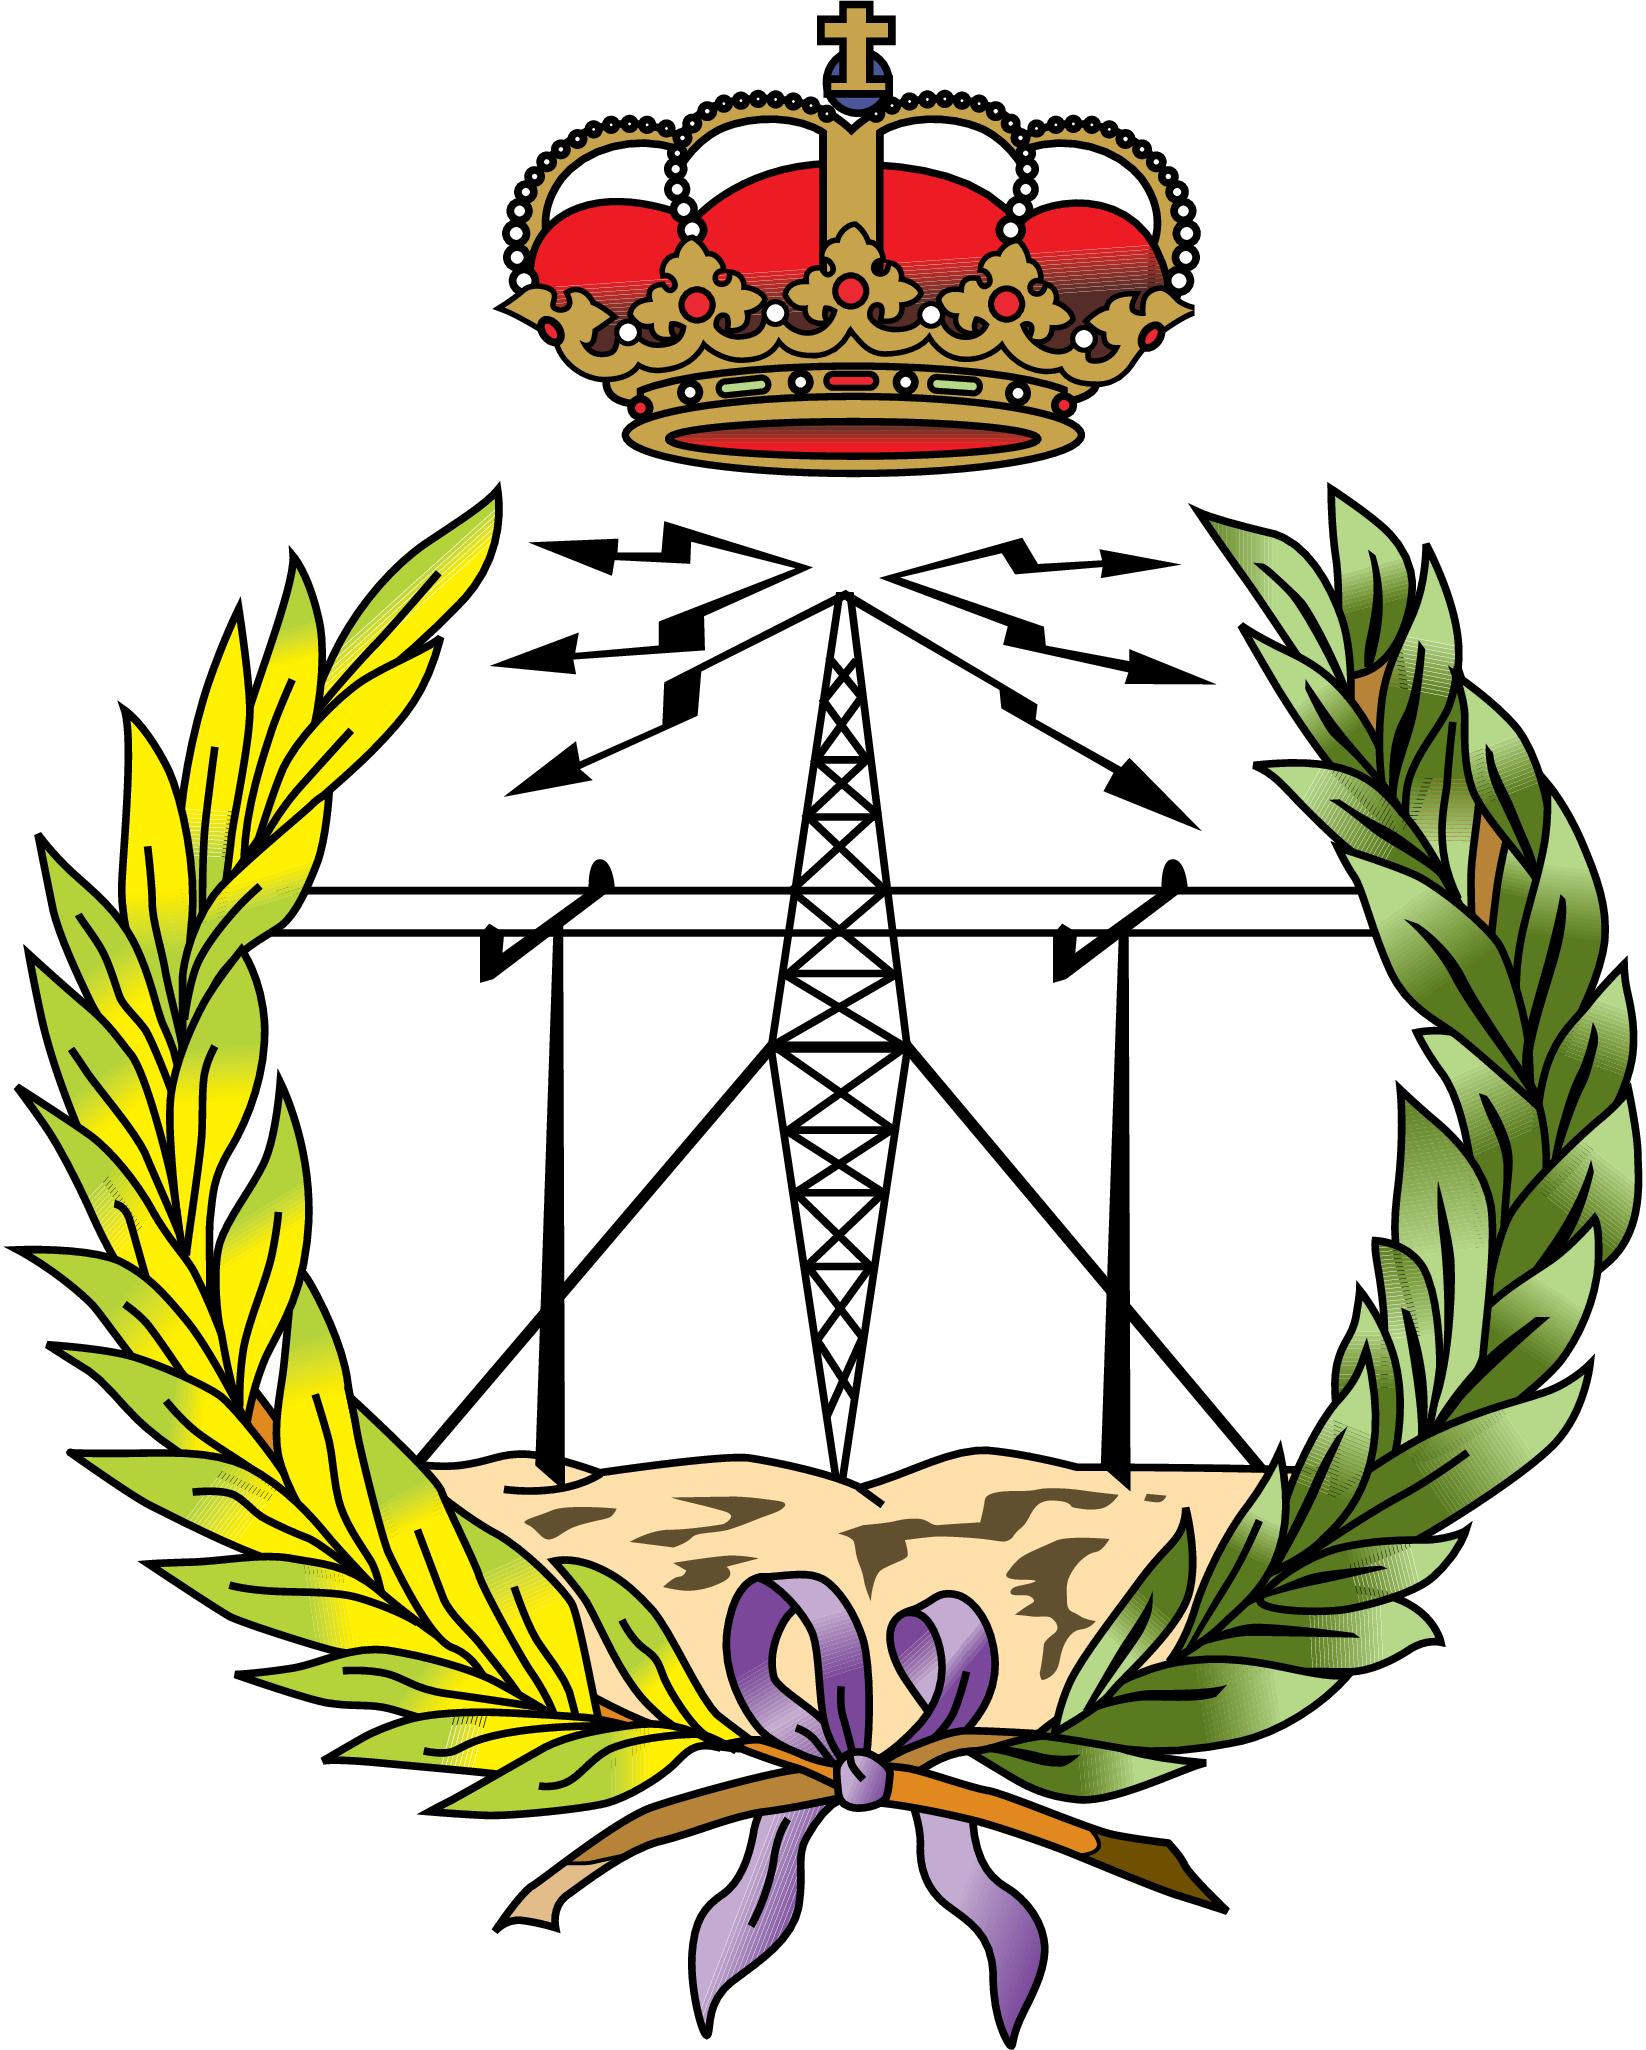
\includegraphics[width=\linewidth]{../../Archivos comunes/etsist_logo.png}
	\end{subfigure}
\end{figure}

\newpage
\phantomsection
\addcontentsline{toc}{section}{Introducción}
\section*{Introducción}
Esta pequeña recopilación de fórmulas, teoremas y demás apuntes de teoría ha sido elaborada durante el primer semestre del curso 2020-2021, en la escuela \href{https://www.etsist.upm.es/}{\textbf{ETSIST}} de la \href{http://www.upm.es/}{\textbf{UPM}} por Javier Rodrigo López, alumno de 2º de Ingeniería de Sonido e Imagen.

Se han tomado como importante referencia los apuntes de \href{https://www.etsist.upm.es/escuela/departamentos/EF/personal?departamento=EFF&idTrabajador=02819b0c47b0eac780a7d0e336d9862b}{Marta Sánchez Agudo}, profesora de Electromagnetismo y Ondas en la ETSIST, descargados desde \href{https://apuntesupmcampussur.wordpress.com/}{este blog}.


\newpage

\setlength{\parskip}{0em}
\tableofcontents
\setlength{\parskip}{0.5em}


\chapter{Oscilaciones}

\section{Movimiento armónico simple}
Una \textbf{oscilación} es un  vaivén o movimiento periódico que realiza una partícula en torno a una posición de equilibrio, debido a una acción perturbadora previa.

Por norma general, se suele colocar el origen de coordenadas ($O$) en la posición de equilibrio del cuerpo en cuestión.

Estudiaremos el movimiento armónico simple (\textbf{\mas} por sus siglas) por ser un caso sencillo, interesante y fácil de extrapolar a otras situaciones.

En el primer apartado, analizaremos la cinemática\footnote{La cinemática es el estudio del movimiento.} necesaria para describir matemáticamente el \mas

El movimiento armónico simple, como su propio nombre indica, realiza un movimiento de carácter armónico\footnote{En este contexto, nos referimos a las funciones seno y coseno} en torno a un punto de equilibrio y a lo largo de un eje (el eje $x$, por ejemplo). \[\boxed{x(t) = A\cdot \sen{\left( \omega t + \phi \right)}}\]

\subsection{\texorpdfstring{\centering Cinemática del \mas}{Cinemática del M.A.S.}}
\begin{multicols}{2}
	
	\subsubsection{Propiedades generales}

	La \textbf{amplitud} $(A)$ es una distancia, y por lo tanto es positiva. Podemos encontrar situaciones en las que no lo encontremos así. Podemos reescribirlo de la siguiente forma: \begin{align*}
		x(t) & = -A\cdot \sen{\left( \omega t + \phi \right)}        \\
		x(t) & = A\cdot \sen{\left( \omega t + \phi \pm \pi \right)}
	\end{align*}

	Como el seno y el coseno son funciones acotadas, la \textbf{elongación} $(x)$ de nuestro \mas \space estará acotada entre $A$ y $-A$. \[\boxed{-A \leq x \leq A}\]

	El \mas\space es un \textbf{movimiento periódico} con periodo $T$. La condición del periodo es que la partícula vuelva al mismo estado en el que se encontraba tras un tiempo $T$, de modo que $x(t) = x(t+T)$.\[\boxed{T=\frac{2\pi}{\omega}}\]

	También se puede definir la \textbf{frecuencia} del movimiento de modo que $f=\frac{1}{T}$.

	Para relacionar el seno y el coseno, recordamos que: \[\sen{\left( \alpha \right)} = \cos{\left( \alpha - \frac{\pi}{2} \right)}\]

	Siendo la $\phi$ \textbf{fase inicial} en un \mas , esto se traduce en que habrá que ajustar la fase un poquito si cambiamos de seno a coseno y viceversa: \[x(t) = \cos{\left( \omega t + \phi ' \right)} \ \longrightarrow \ \boxed{\phi ' = \phi - \frac{\pi}{2}}\]

	\subsubsection{Velocidad y aceleración}

	Como $v=\dv{x}{t}$\, , tenemos que la velocidad de un \mas\space será: \[\boxed{v(t) =A\omega \cdot \cos{\left( \omega t + \phi \right)}}\]

	Cuando el coseno vale 0, el seno vale $1$ ó $-1$, y viceversa.

	Esto quiere decir que la velocidad es \textbf{nula en los extremos} y \textbf{máxima en} $\mathbf{0}$.

	Como $a=\dv{v}{t}$, tenemos que la aceleración de un \mas es: \[\boxed{a(t) = -A\omega ^2 \cdot \sen{\left( \omega t + \phi \right)}}\]

	Sabemos que: \[x(t) = A\cdot \sen{\left( \omega t + \phi \right)}\]
	Así que podemos reescribir la aceleración como: \[\boxed{a = -\omega ^2 \cdot x}\]
\end{multicols}

\subsection{\texorpdfstring{\centering Dinámica del \mas}{Dinámica del M.A.S.}}

\begin{multicols}{2}
	Analizaremos ahora la dinámica\footnote{La dinámica estudia las causas que producen el movimiento.} del \mas


	\subsubsection{Dinámica básica}
	Empezaremos recordando lo que dice la

	Si lo aplicamos a nuestro caso particular, que es el \mas , tenemos que: \[F = ma \qquad \Longrightarrow \qquad F = -m\omega ^2x\]

	Esto signfica que la fuerza es mayor cuanto mayor sea la elongación $x$. O, en otras palabras, la fuerza es mayor cuanto más se acerca a los extremos.

	De aquí es de donde sale la \textbf{Ley de Hooke}:
	\begin{equation} \label{eq:Ley_de_Hooke}
		\boxed{F = -kx}
	\end{equation}
	Vemos que en realidad es lo mismo, ya que:
	\[\left. \begin{matrix*}[r]
			F = -kx \\[5pt]
			F = -m\omega ^2 x
		\end{matrix*}\right\} \longrightarrow k = m\omega ^2\]

	\subsubsection{Ecuación diferencial del \mas}
	Ahora bien, queremos averiguar si existe alguna condición que deba cumplir un movimiento para que sea un \mas \space Podemos hacer lo siguiente: \[F = -kx = ma = m\cdot \dv{^2x}{t^2}\]
	\[-kx = m\cdot \dv{^2x}{t^2} \quad \Longrightarrow \quad \dv{^2x}{t^2} + \frac{k}{m}x = 0 \]

	Esta pequeña ecuación diferencial es la que resume de forma completa el movimiento armónico simple. Si la resuelves, te queda algo así: \[\boxed{x(t) = a\cdot \sen{\left( \omega t \right)} + b\cdot \cos{\left( \omega t \right)}}\]


	Si la reescribimos para que no dependa de $k$ ni de $m$, la \edmas \space queda de la siguiente forma: \[\boxed{\dv{^2x}{t^2} + \omega ^2 x = 0}\]

	\subsubsection{Energía cinética del \mas}
	Particularizando para el \mas , sea: \[x=A\cdot \sen{\left( \omega t + \phi \right)}\]
	Entonces: \[v = A\cdot\cos{\left( \omega t + \phi \right)} \]
	\[E_c = \frac{1}{2}m\omega ^2 A^2 \cdot \cos ^2{\left( \omega t + \phi \right)} \]

	Hacemos el truquito trigonométrico que nos dice que $\sen ^2{\left( \alpha \right)} + \cos ^2{\left( \alpha \right)}= 1$\, , y obtenemos: \[E_c = \frac{1}{2}m\omega ^2 \left[ A^2-A^2 \cdot \sen ^2{\left( \omega t + \phi \right)}\right]\]
	\[\boxed{E_c = \frac{1}{2}k\left( A^2 - x^2 \right)}\]
	Podemos ver que si $x=\pm A$, entonces la energía cinética es nula ($E_c = 0$). Por otro lado, si $x=0$, vemos que la energía cinética es máxima ($E_c = \frac{1}{2}kA^2$).

	\subsubsection{Energía potencial del \mas}
	Tenemos que averiguar si la fuerza que provoca el \mas es conservativa. Por la ley de Hooke (\ref{eq:Ley_de_Hooke}), tenemos que:
	\[\vec{F} = -kx\cdot \vec{u_x}\]
	Lo que debemos hallar es una función potencial para esta fuerza.
	\[\vec{F} = - \grad \cdot \vec{E_p}\]
	\[-kx\cdot \vec{u_x} = -\left( \pdv{E_p}{x} \vec{u_x} + \pdv{E_p}{y}\vec{u_y} + \pdv{E_p}{z}\vec{u_z} \right)\]
	\[\pdv{E_p}{y}\vec{u_y} = \pdv{E_p}{z}\vec{u_z} = 0\]
	\[-kx = -\dv{E_p}{x} \quad \longrightarrow \quad kx\cdot \dd x = \dd E_p\]
	Integramos...
	\[\int{\dd E_p} = \int{kx\cdot \dd x}\]
	\[E_p = \frac{1}{2}kx^2 + C\]

	El origen de la $E_p$ que vamos a elegir es:
	\[E_p(x=0)=0 \quad \longrightarrow \quad C = 0\]
	Entonces, la energía potencial del \mas \space es:
	\[\boxed{E_p = \frac{1}{2}kx^2}\]

\end{multicols}

\section{Composición de movimientos armónicos}
En este apartado, haremos uso de los fasores, así que viene bien que le eches un vistazo en la \autoref{subsec:fasores}.

Sea un \mas \space $x(t) = A\cdot \sen{\left( \omega t + \phi \right)}$, podremos definir un fasor $\vb{A}$ con $\omega$ y $\abs{\vb{A}}$ constantes (si estas dos condiciones no se cumplieran, no sería un \mas ).
\begin{figure}[h!]
	\centering
	\begin{subfigure}[b]{0.65\linewidth}
		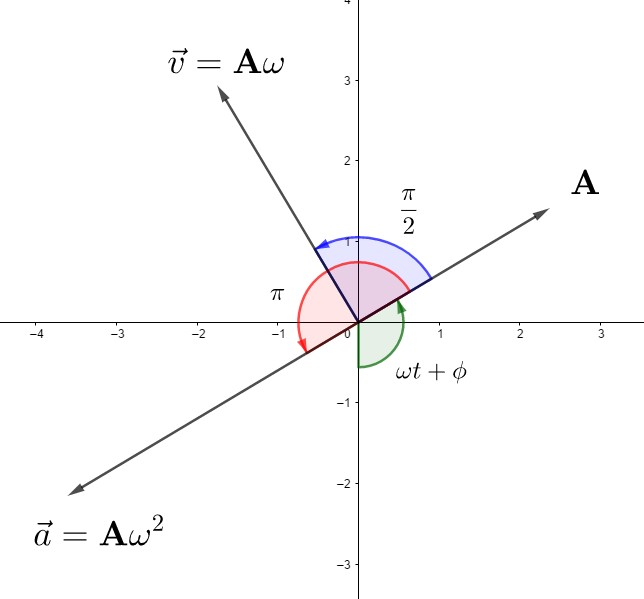
\includegraphics[width=\linewidth]{./Imágenes/aaa.jpg}
	\end{subfigure}
	\caption{Representación del fasor $\vb{A}$.}
\end{figure}


\subsection{\texorpdfstring{Composición de 2 \mas\space paralelos de igual frecuencia}{Composición de 2 M.A.S. paralelos de igual frecuencia}}
Vamos a suponer que ambos se mueven en el eje $x$ para facilitar los cálculos. Entonces, tenemos dos \mas\space $A_1,A_2$ definidos como:
\[
	\begin{matrix}
		x_1 = A_1\cdot \sen{\left( \omega t + \phi _1 \right)} \\
		x_2 = A_2\cdot \sen{\left( \omega t + \phi _2 \right)}
	\end{matrix}
\]

La suma de $\vb{A}_1$ y $\vb{A}_2$ es una suma de vectores típica. En la \autoref{fig:suma_de_vectores} vemos que, para cualquier valor de $t$, el resultado es un fasor $\vb{A}_3$ cuya frecuencia y módulo no varían. Precisamente por eso sabemos que la composición de 2 \mas\space paralelos con igual frecuencia da lugar a otro \mas

\begin{figure}[h!]
	\centering
	\begin{subfigure}[b]{0.6\linewidth}
		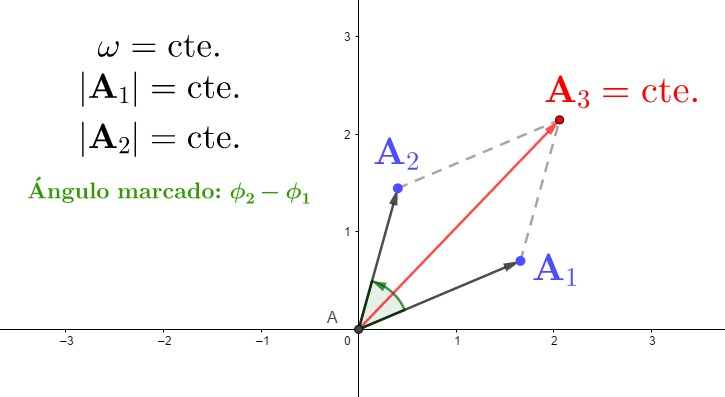
\includegraphics[width=\linewidth]{./Imágenes/aab.jpg}
	\end{subfigure}
	\caption{Suma de fasores.} \label{fig:suma_de_vectores}
\end{figure}

\subsubsection{Calcular la fase}
Sabemos que $\omega $ es constante y que nuestras incógnitas son $A$ y $\phi $.
Si $x_3 = x_1 + x_2$, entonces:
\[A_3\cdot \sen{\left( \omega t + \phi_1 \right)} = A_1\cdot \sen{\left( \omega t + \phi \right)} + A_2\cdot \sen{\left( \omega t + \phi_2 \right)}\]
Además, si usamos la identidad trigonométrica \ref{eq:trig_aaa}, tenemos que:
\[ \begin{split}
		A_3\cdot \sen{\left( \omega t \right)}\cos{\left( \phi _3 \right)}+ A_3\cdot \cos{\left( \omega t \right)}\sen{\left( \phi _3 \right)} = A_1\cdot \sen{\left( \omega t \right)}\cos{\left( \phi _1 \right)}+ A_1\cdot \cos{\left( \omega t \right)}\sen{\left( \phi _1 \right)} \\
		+ A_2\cdot \sen{\left( \omega t \right)}\cos{\left( \phi _2 \right)}+ A_2\cdot \cos{\left( \omega t \right)}\sen{\left( \phi _2 \right)}
	\end{split}
\]

Podemos dividir esta ecuación en dos partes para verlo mejor, sacando $\sen{\left( \omega t \right)}$ y $\cos{\left( \omega t \right)}$ como factores comunes de las siguientes expresiones respectivamente:
\[\begin{matrix*}[l]
		\circledNumber{1}\  A_3\cdot \cos{\left( \phi _3 \right)} = A_1\cdot \cos{\left( \phi _1 \right)} + A_2\cdot \cos{\left( \phi _2 \right)} \\[5pt]
		\circledNumber{2}\  A_3\cdot \sen{\left( \phi _3 \right)} = A_1\cdot \sen{\left( \phi _1 \right)} + A_2\cdot \sen{\left( \phi _2 \right)}
	\end{matrix*}\]

De este modo, es mucho más fácil ver que:
\[\frac{\circledNumber{2}}{\circledNumber{1}} = \frac{A_3\cdot \sen{\left( \phi _3 \right)}}{A_3\cdot \cos{\left( \phi _3 \right)}} = \boxed{ \tg{\left( \phi_3 \right)} =\frac{A_1\cdot \sen{\left( \phi _1 \right)} + A_2\cdot \sen{\left( \phi _2 \right)}}{A_1\cdot \cos{\left( \phi _1 \right)} + A_2\cdot \cos{\left( \phi _2 \right)}}}\]

Ya tenemos la fase de nuestro \mas \space Si hacemos la arcotangente, nos dará dos soluciones posibles, así quetendremos que fijarnos en qué cuadrante está la fase de los otros para escribirla correctamente. Puedes revisar cómo se calcula la arcotangente en el apartado (insertar referencia).

\subsubsection{Calcular la amplitud}
Ya que tenemos calculada la fase, ahora calcularemos la amplitud. El camino a seguir será el siguiente:
\[\boxed{\circledNumber{1}^2 + \circledNumber{2}^2}\]
El resultado de esta operación debería ser algo como:
\[\begin{split}
		A_3^2 \cdot \cos ^2\left( \phi_3 \right) + A_3^2 \sen ^2\left( \phi_3 \right) = A_1^2 \cos ^2\left( \phi_1 \right) + A_1^2 \sen ^2\left( \phi_1 \right)\\ + A_2^2 \cos ^2\left( \phi_2 \right) + A_2^2 \sen ^2\left( \phi_2 \right) \\ +2A_1A_2\cos \left( \phi_1 \right)\cos \left( \phi_2 \right)\\+2A_1A_2\sen \left( \phi_1 \right)\sen \left( \phi_2 \right)
	\end{split}\]
Simplificamos:
\[A_3^2 = A_1^2 + A_2^2 + 2A_1A_2 \underbrace{\left[ \sen \left( \phi_1 \right)\sen \left( \phi_2 \right) + \cos \left( \phi_1 \right)\cos \left( \phi_2 \right) \right]}_{\cos \left( \phi _2 - \phi _1 \right)\  = \ \cos \left( \delta \right)\qquad \! } \]

Vemos que $\delta$ vale $\phi _2 - \phi _1$, pero también vale $ \phi _1 - \phi _2 $, ya que el coseno es una función par y esto no afecta al resultado. En otras palabras, $\delta$ es la \textbf{diferencia de fase}.

Tenemos entonces que la amplitud vale:
\[\boxed{A = \sqrt{A_1^2+A_2^2+2A_1A_2 \cos \left( \delta \right)}}\]

\subsection{\texorpdfstring{Composición de 2 \mas\space paralelos de diferente frecuencia}{Composición de 2 M.A.S. paralelos de diferente frecuencia}}
En este caso, al no tener misma frecuencia, el resultado de la composición de los dos movimientos no será un \mas , así que trabajaremos con lo que tenemos, que sigue siendo:
\[x = x_1 + x_2\]
\subsection{\texorpdfstring{Composición de 2 \mas\space perpendiculares de igual frecuencia}{Composición de 2 M.A.S. perpendiculares de igual frecuencia}}
Para simplificar, usaremos las direccion de los ejes $x,y$.
\[\begin{matrix*}[l]
		x = A \cdot \sen\left( \omega t + \phi_1 \right)\\
		y = B \cdot \sen\left( \omega t + \phi_2 \right)
	\end{matrix*}\]

Definimos al igual que antes el desfase $\delta$ de modo que:
\[\delta = \left\{ \begin{matrix*}[l]
		\phi_2 - \phi_1\\
		\phi_1 - \phi_2
	\end{matrix*} \right. \]

Ahora, pasaremos a calcular esta composición, y diferenciamos dos situaciones para realizar el cálculo.

\subsubsection{Movimientos en fase}
En esta situación, tenemos que $\phi_1 = \phi _2$. Por lo tanto, $\delta = 0$. Ambos movimientos están en fase.

Seguiremos una serie de pasos:
\begin{enumerate}
	\item Comprobar si \textbf{la trayectoria es una recta}. De lo contrario, no sería un \mas

	      Como las fases iniciales son iguales, tenemos que:
	      \[\left. \begin{matrix}
			      x = A \cdot  \sen\left( \omega t + \phi_1\right) \\
			      y = B \cdot  \sen\left( \omega t + \phi_1 \right)
		      \end{matrix} \right\} \longrightarrow \frac{x}{A} = \frac{y}{B} \Rightarrow \boxed{y = \frac{B}{A}x}\]
	      Tenemos una pendiente $\frac{B}{A}$ positiva, ya que $A,B$ son amplitudes. Por ahora, tiene pinta de que va a ser un \mas , ya que el movimiento siempre se realiza en la misma dirección.

	\item Se debe poder escribir \textbf{la distancia al centro de oscilación} como $A\cdot \sen\left( \omega t + \phi \right)$.

	      Si lo calculamos mediante el vector posición $\vec{r}$, tal y como muestra la figura (insertar referencia), tenemos que:
	      \begin{align*}
		      r & = \sqrt{x^2+y^2}                                                                                             \\
		      r & = \sqrt{A^2\cdot \sen ^2\left( \omega t + \phi_1 \right) + B^2\cdot \sen ^2\left( \omega t + \phi_1 \right)} \\
		        & = \sen\left( \omega t + \phi_1 \right)\underbrace{\sqrt{A^2+B^2}}_{r_0}                                      \\
		      r & = r_0\cdot \sen\left( \omega t + \phi_1 \right) \quad \longrightarrow \quad \text{Es un \mas}
	      \end{align*}

\end{enumerate}
\subsubsection{Movimientos en oposición de fase}
Cuando los movimientos están en oposición de fase, significa que $\delta = \pm \pi$. Por lo tanto, $\phi_2 = \phi_1 \pm \pi$.
\begin{enumerate}
	\item Hallamos la \textbf{trayectoria}.
	      \[\begin{matrix*}[l]
			      x = A \cdot \sen\left( \omega t + \phi_1 \right)\\
			      y = B \cdot \sen\left( \omega t + \phi_1 \pm\pi \right)
		      \end{matrix*}\]

	      Sabemos que $\sen\left( \alpha \right) = - \sen\left( \alpha \pm\pi \right)$, por lo tanto:
	      \[y = -B\cdot \sen\left( \omega t + \phi_1 \right)\]

	      A partir de aquí, podemos operar como antes: \[\left. \begin{matrix}
			      x = A \cdot  \sen\left( \omega t + \phi_1\right) \\
			      y = -B \cdot  \sen\left( \omega t + \phi_1 \right)
		      \end{matrix} \right\} \longrightarrow \frac{x}{A} = -\frac{y}{B} \Rightarrow \boxed{y = -\frac{B}{A}x}\]

	      Nos encontramos con la misma situación que tuvimos con los movimientos en fase. Sin embargo, esta vez tenemos una recta de pendiente $-\frac{B}{A}$ negativa.

	\item Compronbamos que se pueda definir la \textbf{distancia al centro de oscilación}, al igual que antes. El módulo del vector posición queda definido en este caso como:
	      \[r = \underbrace{\sqrt{A^2+B^2}}_{r_0}\cdot \sen\left( \omega t + \phi_1 \right)\quad \longrightarrow \quad \text{Es un \mas }\]
\end{enumerate}
\subsubsection{Movmientos en cuadratura}
Un movimiento está en cuadratura con otro si la diferencia de sus fases es $\delta = \frac{\pi}{2}$. Definimos entonces las fases iniciales de cada movimiento como $\phi_2 = \phi_1 \pm \frac{\pi}{2}$ (aunque vamos a hacer la demostración con $+\frac{\pi}{2}$ para simplificar el desarrollo).

\begin{enumerate}
	\item Hallamos la \textbf{trayectoria}.
	      \[\begin{matrix*}[l]
			      x = A \cdot \sen\left( \omega t + \phi_1 \right)\\
			      y = B \cdot \sen\left( \omega t + \phi_1 +\frac{\pi}{2}\right)
		      \end{matrix*}\]

	      Por la relación entre el seno y el coseno (\ref{eq:trig_aae}), sabemos que $\sen\left( \alpha + \frac{\pi}{2} \right) = \cos\left( \alpha \right)$. Por lo tanto:
	      \[y = B\cdot \cos\left( \omega t + \phi_1 \right)\]

	      Si elevamos todo al cuadrado, podremos obtener una solución:
	      \[\begin{matrix*}[l]
			      x^2 = A^2 \cdot \sen^2\left( \omega t + \phi_1 \right)\\
			      y^2 = B^2 \cdot \cos^2\left( \omega t + \phi_1 \right)
		      \end{matrix*}\]

	      Además, por la relación fundamental de la trigonometría (\ref{eq:trig_aad}), sabemos que $\sen^2 \left( a \right) + \cos^2 \left( a \right) = 1$, por lo que podemos establecer una relación entre $x$ e $y$:
	      \[\frac{x^2}{A^2} + \frac{y^2}{b^2} = 1\]

	      Esta ecuación, representa la trayectoria de una elipse centrada en el origen y con los semiejes en los ejes de coordenadas.

	      Hemos comprobado que, en este caso, el resultado no es un \mas\space No podemos decir que el movimiento sea unidireccional. Para caracterizar completamente este movimiento, debemos averiguar en qué \textbf{sentido} se recorre la elipse.
	      \[\left. \begin{matrix*}[l]
			      x = A \cdot \sen\left( \omega t + \phi_1 \right)\\
			      y = B \cdot \cos\left( \omega t + \phi_1 \right)
		      \end{matrix*}\right\} \quad \longrightarrow \quad \vec{r} = x\vec{u_x} + y\vec{u_y}\]
	      \[\boxed{\vec{r} = A \cdot \sen\left( \omega t + \phi_1 \right) \vec{u_x} + B \cdot \cos\left( \omega t + \phi_1 \right) \vec{u_y}}\]

	      El vector velocidad es siempre tangente a la trayectoria. Lo que haremos será analizar un punto cualquiera de la elipse (ver figura [referencia]) y ver "qué pinta tiene".
	      \[\left. \begin{matrix*}[r]
			      \displaystyle{v_x = \dv{x}{t} = A\omega \cdot \cos\left( \omega t + \phi_1 \right)}\\[10pt]
			      \displaystyle{v_y = \dv{y}{t} = -B\omega \cdot \sen\left( \omega t + \phi_1 \right)}
		      \end{matrix*}\right\} \quad \longrightarrow \quad \vec{v} = v_x\vec{u_x} + v_y\vec{u_y}\]
	      \[\boxed{\vec{v} = A\omega \cdot \sen\left( \omega t + \phi_1 \right) \vec{u_x} - B\omega \cdot \cos\left( \omega t + \phi_1 \right) \vec{u_y}}\]

	      Si cogemos un punto fácil, como el extremo de un semieje, podemos ver cómo se comporta el movimiento. Vamos a coger el punto $(0,B)$, de modo que la velocidad solo tendrá la componente $x$, como se puede observar en la figura [falta referencia].

	      Diremos que en el instante $t = t_0$ nos encontraremos en la posición $(0,B)$.
	      \begin{align*}
		      x = 0 = A \cdot \sen\left( \omega t_0 + \phi_1 \right) \quad \longrightarrow\quad   \sen\left( \omega t_0 + \phi_1 \right) = 0 \\
		      y = B = B \cdot \cos\left( \omega t_0 + \phi_1 \right)\quad \longrightarrow\quad   \cos\left( \omega t_0 + \phi_1 \right) = 1
	      \end{align*}

	      Si sustituimos esto en las componentes de la velocidad, tenemos que:
	      \begin{align*}
		      v_x = A\omega \cdot \cancelto{1}{\cos\left( \omega t_0 + \phi_1 \right)} = A\omega \\
		      v_y = -B\omega \cdot \cancelto{0}{\sen\left( \omega t_0 + \phi_1 \right)} = 0
	      \end{align*}

	      Podemos ver que la componente $v_x$ es positiva en el punto $(0,B)$, por lo que este movimiento se produce en sentido horario.
\end{enumerate}

\subsection{Caso general}
Si realizas los cálculos para una diferencia de fase $\delta$ arbitraria, obtendrás que la trayectoria del movimiento resultante será la siguiente:
\[\boxed{\frac{x^2}{a^2} + \frac{y^2}{b^2} - \frac{2xy}{AB}\cos\left( \delta \right) = \sen^2\left( \delta \right)}\]
Esto se traduce en una elipse centrada en el origen, pero cuyos semiejes no tienen por qué coincidir con los ejes de coordenadas. Puedes verlo mejor en la figura [falta referencia].

\section{Oscilaciones amortiguadas y forzadas}
\subsection{Movimiento oscilatorio amortiguado}

Un oscilación amortiguada es parecido a un \mas , pero en este caso la amplitud $A$ no es constante.

Este movimiento es resultado de la acción de dos fuerzas diferentes:
\begin{enumerate}
	\item La \textbf{fuerza elástica} que produce un \mas\space y que es descrita por la ley de Hooke (\ref{eq:Ley_de_Hooke}).
	      \[F_e = -kx\]
	\item Una \textbf{fuerza amortiguadora}.
	      \[F_\lambda = -\lambda v\]
\end{enumerate}

Vemos que la fuerza total $F_T$ aplicada a la partícula, relacionada con la segunda ley de Newton (\ref{eq:segunda_ley_Newton}), es la siguiente:
\begin{align*}
	F_T = F_e + F_\lambda = ma \\
	-kx-\lambda v=ma
\end{align*}
Como $a=\dv[2]{x}{t}, v = \dv{x}{t}$, entonces la \textbf{ecuación diferencial del movimiento oscilatorio amortiguado} es la siguiente:
\[m\dv[2]{x}{t} + \lambda \dv{x}{t} + kx = 0\]
Aunque es frecuente escribirla así:
\[\boxed{\dv[2]{x}{t} + 2\gamma \dv{x}{t} + \omega_o^2x = 0}\]
Donde $2\gamma=\frac{\lambda}{m}$ y $\omega_o^2=\frac{k}{m}$. En esta ecuación, $omega_o$ representa la frecuencia que tendría el \mas\space si no hubiera amortiguamiento.

Las \textbf{soluciones} de esta ecuación diferencial dependerán de la relación entre $\gamma$ y $\omega_o$.
\begin{enumerate}[label=\alph*)]
	\item Si $\gamma < \omega_o$ hay poco amortiguamiento. Estamos en \textbf{régimen subamortiguado}.
	      \[\boxed{x = Ae^{-\gamma t}\cdot \sen\left( \omega t+ \phi \right)}\]
	      Podemos ver que la amplitud no es constante, disminuye con el tiempo.

	      También encontramos que la frecuencia no es la misma que en un \mas , sino que es ligeramente inferior:
	      \[\omega = \sqrt{\omega_o^2 - \gamma^2}\, \quad \longrightarrow \quad  \omega < \omega_o\]
	\item Si $\gamma \sim \omega_o$ se dice que estamos en \textbf{régimen crítico}.
	      \[x=\left( A+Bt \right)e^{-\gamma t}\]
	      Vemos que en este movimiento no se produce oscilación. (Ver figura [falta referencia])

	\item Si $\gamma < \omega_o$ estamos en \textbf{régimen sobreamortiguado}.
	      \[x=\left( Ae^{t\sqrt{r^2-\omega_o^2}} +Be^{-t\sqrt{\gamma^2-\omega_o^2}}\right)\]
	      Este se parece al movimiento en régimen crítico, pero tarda más en llegar a la posición de equilibrio.
\end{enumerate}

\subsubsection{Energía en movimientos oscilatorios amortiguados}
Se sigue cumpliendo que $E_T = E_c + E_p$.
\[E_T = \frac{1}{2}mv^2 + \frac{1}{2}kx^2\]

Sin embargo, este valor ya no es constante.
\[\dv{E_T}{t} = \frac{1}{2}m\cdot 2v\dv{v}{t} + \frac{1}{2}k\cdot 2x\dv{x}{t}\]

De la ecuación donde relacionamos la segunda ley de Newton y las fuerzas que se aplican a este tipo de movimiento (un poco más arriba en esta misma sección), tenemos que:
\[-kx-\lambda v=ma \quad \longrightarrow \quad ma+kx=-\lambda v\]

Por lo que podemos sustituir:
\begin{align*}
	\dv{E_T}{t} & = mva + kxv = v\underbrace{\left( ma+kx \right)}_{-\lambda v} = -\lambda v^2
\end{align*}
\[\boxed{\dv{E_T}{t} = -\lambda v^2}\]
A esta expresión la denominamos \textbf{potencia amortiguadora}.

Podemos apreciar que la variación de la energía total de este movimiento es negativa. Esto se traduce en que el sistema \textbf{pierde energía}.

\subsection{Movimiento oscilatorio forzado}
Cuando aplicamos una fuerza que compensa a la fuerza amortiguadora $F_\lambda$ conseguimos un movimiento oscilatorio forzado. A esta fuerza la llamaremos \textbf{fuerza impulsora}.
\[F_f=F_0\cdot \cos\left( \omega_ft \right)\]
Usamos el coseno porque esto facilitará los cálculos. Si la relacionamos con la segunda ley de Newton (\ref{eq:segunda_ley_Newton}), tenemos que:
\[F_T = -kx-\lambda v + F_0\cdot \cos\left( \omega_ft \right) = ma\]
Si lo podemos en forma diferencial:
\[-kx -\lambda \dv{x}{t} + F_0\cdot \cos\left( \omega_ft \right) = m\dv[2]{x}{t}\]

Y si además reemplazamos $\gamma$ y $\omega_o$\footnote{Recordamos que $2\gamma = \frac{\lambda}{m}$ y que $\omega_o^2 = \frac{k}{m}$} en la ecuación y tenemos:
\[\boxed{\dv{x}{t} + 2\gamma \dv{x}{t} + \omega_o^2x = F_o\cdot \cos\left( \omega_f t \right)}\]

La solución a esta ecuación diferencial es:
\[x = A\cdot \sen\left( \omega_ft-\alpha \right)\]
La fase $\alpha$ se encuentra restando por facilidad a la hora de operar. Si derivamos esta expresión, la sustituimos en la ecuación diferencial y despejas $A$ y $\alpha$ obtienes lo siguiente:
\[A=\frac{\displaystyle{\frac{F_0}{m}}}{\sqrt{\left( \omega_f^2-\omega_o^2 \right)^2 + 4\gamma ^2\omega_f^2}}\qquad \qquad \tg \left( \alpha \right) = \frac{\omega_f^2-\omega_o^2}{2\gamma\omega_f}\]
$\omega_o$ y $m$ son características de cada sistema. Además $A$ es función de $\omega_f$ y de $\gamma$.

\subsubsection{Resonancia en amplitud}
Si $\gamma$ es constante, la amplitud tomará diferentes valores (representados en la figura [falta referencia]) de forma que habrá un valor de $\omega_f = \omega_R$ al que llamamos \textbf{frecuencia de resonancia} para el cual la amplitud es máxima. Este estado se denomina \textbf{resonancia en amplitud}.

Si derivamos $A$ e igualamos a cero, podemos obtener ese valor, que es:
\[\boxed{\omega_R = \sqrt{\frac{k}{m}-\frac{\lambda^2}{2m^2}}}\]

De modo que la amplitud máxima sería:
\[\boxed{A = \frac{\sfrac{F_0}{m}}{2\gamma \sqrt{\omega_o^2-\gamma^2}}}\]

Este valor dependerá de cuánto amortiguamiente tenga el movimiento.

\subsubsection{Resonancia en energía}
También se puede conseguir otro tipo de resonancia diferente, que es la \textbf{resonancia en energía}. Cuando $E_c$ es máxima, la velocidad $v$ también es máxima.

\[v=\dv{x}{t} = \underbrace{A\omega_f}_{v_o}\cdot \cos\left( \omega_fy + \phi \right)\]

Luego, si se consigue $v\subtext{máx}$ también se conseguirá
$v_{o\, \text{máx}}$. Como $v_o$ es:
\[v_o = \frac{\omega_f\frac{F_o}{m}}{\sqrt{\left( \omega_f^2-\omega_o^2 \right)^2+4\gamma^2\omega_f^2}}\]

Si derivamos esa expresión, llegaremos a la conclusión de que:
\[v_{o\,  \text{máx}}\quad \longrightarrow \quad \boxed{\omega_f=\omega_o = \frac{k}{m}}\]

En estas condiciones no se puede conseguir la amplitud máxima, pero sí que se puede conseguir la \textbf{máxima transferencia de energía} en el sistema. Conseguimos que la velocidad esté en fase con la fuerza aplicada. Cuanto más pequeño es el amortiguamiento, más se parecen las frecuencias que hacen que la amplitud y la energía del sistema sean máximas.



\chapter{Ondas en medios elásticos}

\section{Características. Función y ecuación de ondas}

\subsubsection{Definición de onda}
Una onda es una propagación de una perturbación a lo largo de un medio. Se propagan energía y momento, pero no materia.

\subsubsection{Función de onda}
Podemos describir matemáticamente el comportamiento de una onda mediante la denominada \textbf{función de onda}:
\[\Psi\left(\vec{r},t\right)\]
Donde $\vec{r}$ es el vector posición donde queremos comprobar qué estado tiene esa perturbación y $t$ es el instante de tiempo en el cual lo observamos.

\subsubsection{Frente de onda}
Es el \textbf{lugar geométrico} de los puntos del espacio que son alcanzados de manera simultánea por la onda y que, en consecuencia, se encuentran en el mismo estado de perturbación.

Los frentes de onda son perpendiculares a la dirección de propagación de la onda.

\subsection{Clasificación de las ondas en función del frente de onda}
\begin{myenumerate}
	\item \textbf{Ondas planas.} El frente de onda es un plano.
	\item  \textbf{Ondas cilíndricas.} Los frentes de onda son cilindros.
	\item \textbf{Ondas esféricas.} Los frentes de onda son esferas. Este tipo de ondas tienen lugar cuando \textbf{el foco es puntual}.
\end{myenumerate}

\subsection{Clasificación de las ondas en función del movimiento}
\begin{myenumerate}
	\item \textbf{Ondas transversales.} Suceden cuando la perturbación es perpendicular a la dirección de propagación.
	\item  \textbf{Ondas longitudinales.} Suceden cuando la perturbación es paralela a la direcciónde propagación.
	\item \textbf{Ondas complejas.} Suceden cuando la perturbación es una combinación de perturbaciones longitudinal y transversal.
\end{myenumerate}

En esta asignatura nos ocuparemos de las ondas mecánicas, ya que son las más sencillas desde el punto de vista matemático, sobre todo las ondas armónicas que estudiaremos en la próxima sección.

\section{Ondas armónicas}

Las \textbf{ondas armónicas} son aquellas donde cada punto medio realiza un \mas\space Se pueden estudiar ondas más complejas producto de la superposición de ondas armónicas.

\subsection{Función de onda unidimensional}
Para provocar una onda armónica en una cuerda podemos provocar un \mas\space en el extremo de la misma, como se indica en la figura [falta referencia].

Como necesitamos un sistema de referencia, situaremos la dirección de propagación de la onda con el eje $x$ y a la dirección del \mas\space con el eje $y$, por simplicidad. La posición de equilibrio del foco será el origen.

El foco realiza un movimiento armónico simple, descrito por la ecuación:
\[y(t) = \Psi_o\cdot \sen\left( \omega t + \phi \right)\]

Si observamos el punto $P$ de la figura [falta referencia, misma que antes], podemos preguntarnos: ¿cuánto tiempo hay que esperar para que el punto $P$ también se mueva como el foco? Pues ese tiempo será $t'$ y obtendremos así:
\[t' = \frac{x}{v}\]
Luego, $P$ realiza un \mas :
\[\Psi _o\cdot \sen\left[ \omega \left( t-t' \right) + \phi \right]\]

También podemos poner la ecuación anterior de la siguiente manera:
\[\Psi _o\cdot \sen\left[ \omega \left( t-\frac{x}{v} \right) + \phi \right]\]

Ahora la función ya depende de $x$ y $t$. Esta es la función de onda, donde los parámetros son \textbf{tiempo} y \textbf{distancia al foco}:
\[\Psi \left( x,t \right) = \Psi_o\cdot \sen\left[ \omega \left( t-\frac{x}{v} \right) +\phi\right]\]

De todas formas, normalmente no se escribe así, sino que se utiliza la propiedad $\omega = \frac{2\pi}{T}$ y se sustituye el producto $Tv$ por el símbolo $\lambda$, que representa la \textbf{longitud de onda} (distancia que recorre la onda en un periodo). Y, para acomodarlo un poco más si cabe, definimos el parámetros $k$ al que llamamos \textbf{número de onda}, y vale $k=\frac{2\pi}{\lambda}$.

Además, podemos establecer una relación entre la velocidad angular y un nuevo parámetro llamado \textbf{número de onda} $(k)$:

\[\left. \begin{matrix*}[l]
		\displaystyle{\omega = \frac{2\pi}{T}}\\[15pt]
		\displaystyle{k=\frac{2\pi}{\lambda}}
	\end{matrix*}\right\} \quad \longrightarrow \quad \omega T = k\lambda \quad \longrightarrow \quad \frac{\lambda}{T} = \boxed{v = \frac{\omega}{k}}\]

Siendo $v$ la velocidad de propagación de la onda.

Esto nos permite reescrbibir un poco la ecuación, \textbf{obteniendo así la ecuación del frente de onda para una dimensión}:
\[\boxed{\Psi\left(x,t\right) = \Psi_o\cdot \sen\left( \omega t -kx + \phi \right)}\]




\subsubsection{Comportamiento temporal}
La función de onda describe el comportamiento temporal de la onda. Es decir, si fijo $x$ y lo represento gráficamente en función del tiempo, podemos observar que ese punto $x$ que hemos fijado realiza un \mas

Los parámetros que describen el comportamiento temporal en la función de onda son el \textbf{periodo} $(T)$ y la \textbf{velocidad angular} $(\omega )$.

\subsubsection{Comportamiento espacial}
El comportamiento espacial viene descrito por los parámetros \textbf{número de onda} $(k)$ y \textbf{longitud de onda} $(\lambda )$. Si fijamos el tiempo $t$ a un instante concreto, podemos representar gráficamente una ``imagen'' de la cuerda en ese instante (ver figura [falta referencia]).

\subsection{Función de onda armónica}
En una cuerda, la función armónica es la que acabamos de sacar:
\[\boxed{\Psi\left(x,t\right) = \Psi_o\cdot \sen\left( \omega t -kx +\phi \right)}\]

Si hablamos de los focos:
\[\left\{ \begin{matrix}
		\Psi_1 = \Psi_{o1}\sen\left( \omega t - kx + \phi_1 \right) \\
		\Psi_2 = \Psi_{o2}\sen\left( \omega t - kx + \phi_2 \right)
	\end{matrix}\right. \]

Podemos disntiguir varias situaciones diferentes:
\begin{itemize}
	\item $\Psi_1$ emite \textbf{retrasado} con respecto a $\Psi_2$ si se cumple que $\boxed{\pi<\phi_1-\phi_2<2\pi}$
	\item $\Psi_1$ emite \textbf{adelantado} con respecto a $\Psi_2$ si se cumple que $\boxed{0<\phi_1-\phi_2<\pi}$
	\item $\Psi_1$ y $\Psi_1$ emiten \textbf{en fase} si se cumple que $\boxed{\phi_1-\phi_2=0}$
	\item $\Psi_1$ y $\Psi_1$ emiten \textbf{en oposición de fase} si se cumple que $\boxed{\phi_1-\phi_2=\pm \pi}$
\end{itemize}

Esta ecuación nos puede ser de utilidad también para ciertas ondas tridimensionales.

Un ejemplo sería un pistón (algo que se mueve en el interior de un tubo hueco), que genera una variación de presión en las moléculas del aire (ver figura [falta referencia]). Todas las moléculas de aire que están a la misma distancia del foco realizan el mismo \mas\space Por cómo es el tubo, el frente de ondas es aproximadamente un plano perpendicular al tubo, por lo que solo deberíamos tener en cuenta el eje $x$ y la función de onda resultaría:
\[\Psi\left(\vec{r},t\right) = \Psi_o\cdot \sen\left( \omega t - k \vec{r} \vec{u_x} + \phi \right)\]



\section{Ondas en dos y tres dimensiones}
\subsection{Función de onda plana}
¿Qué ocurre si la dirección de propagación es una cualquiera? Supongamos una dirección de propagación $\vec{u}$.

Solo nos interesa la distancia desde el punto hasta el foco según la dirección de propagación.
\[\vec{r}\cdot \vec{u}\quad \quad \Psi_o\sen\left( \omega t -k\vec{r}\cdot \vec{u} + \phi \right)\]

Definimos un nuevo vector $\vec{k} = k\vec{u}$ llamado \textbf{vector de onda}. Entonces la función de onda plana queda de la siguiente forma:
\[\Psi\left(\vec{r},t\right) = \Psi_o\sen\left( \omega t - \vec{k}\cdot \vec{r} + \phi \right)\]

Nótese que la onda, a pesar de propagarse en un medio tridimensional, se considera unidimensional porque la dirección de propagación es unidimensional.

\subsection{Función de onda esférica}
Sabemos que en una onda esférica el foco es puntual. Como la dirección de propagación es radial, nos interesan las coordenadas esféricas. El vector $\vec{u_r}$ será la \textbf{dirección radial}. Por lo tanto:
\[\begin{matrix*}[l]
		\vec{k} = k\vec{u_r}\\[5pt]
		\vec{r} = r\vec{u_r}
	\end{matrix*} \]
Y, por consiguiente:
\[\vec{k}\cdot \vec{r} = kr\]
La fase sería entonces $\omega t -kr +\phi$, de modo que deja de tener carácter vectorial. Debemos tener en cuenta que la amplitud es función de la distancia al foco:
\[\Psi_o(r)\]

\subsection{Función de onda cilíndrica}
Se utilizan coordenadas cilíndricas de propagación, por medio del vector director $\vec{u_\rho}$:
\[\begin{matrix*}[l]
		\vec{k} = k\vec{u_\rho}\\[5pt]
		\vec{r} = r\vec{u_\rho}
	\end{matrix*}\]

Al igual que en las ondas esféricas, vemos que $\vec{k}\cdot \vec{r} = kr$, por lo que la fase tampoco tiene carácter vectorial y la amplitud es de nuevo función de la distancia al eje:
\[\Psi_o'(\rho )\]

\section{Intensidad y nivel de intensidad}
\subsection{Intensidad de una onda}
La intensidad de una onda se define como la cantidad de energía por unidad de tiempo que se propaga por unidad de superficie perpendicular a la dirección de propagación.
\[\text{Intensidad} = \frac{\sfrac{\text{Energía}}{\text{Tiempo}}}{\text{Superficie}} = \frac{\text{Potencia}}{\text{Superficie}} \qquad [I ] = \frac{\omega}{m^2}\]

Donde la potencia es la \textbf{potencia de emisión del foco}. Este parámetro describe cómo se reparte la potencia del foco en el frente de onda.

Para cualquier onda, lo podemos generalizar así:
\[\I =\rho_E \cdot v\]
Donde $\rho_E$  es la \textbf{densidad de energía del medio} $[\J\cdot \m^{-n}]$ para un medio de dimensión $n$. Si el medio es unidimensional, se dice que la densidad es lineal. Además, las unidades en ese caso serían $[\J\cdot \m^{-1}]$.

Vamos a comprobar que $I = \rho_E \cdot v$. Nos fijamos en la figura [falta referencia] para intentar resolver el problema. En $\dd{t}$ pasa una energía $\dd{E}$ por el ``trocito'' de tubo de anchura $\dd{l}$. ¿Cómo calcularíamos la intensidad?

Teniendo en cuenta que la velocidad de propagación se puede escribir como $v = \dv{l}{t}$, podemos sustituir en la ecuación de la intensidad:
\[I = \frac{\dv{E}{t}}{S} \quad \Longrightarrow \quad I = \frac{\dd{E}}{S\cdot \dd{l}}\cdot v = \dv{E}{v}\cdot v = \rho_E\cdot v\]

Para ondas armónicas, se cumple que:
\[I\sim \Psi_o^2\]

Esto lo podemos comprobar para el caso de ondas en una cuerda. Como aparece en la figura [falta referencia], vamos a coger un ``trocito de cuerda'' $(\dd{m})$ que realizará un \mas\space Este tendrá una energía:
\[\dd{E} = \frac{1}{2}\dd{m}\omega^2\Psi_o^2\]

Sabemos que $\dd{m} = \mu \dd{l}$, donde $\mu$ es la \textbf{densidad lineal de masa}, y también sabemos que $I=\rho_E\cdot v$, por lo que podemos desarrollar:
\[\dd{E} = \frac{1}{2}\omega^2 \mu \dd{l}\Psi_o^2 \quad \longrightarrow \quad \dv{E}{l} = \frac{1}{2}\omega^2\mu\Psi_o^2 = \rho _E\]

\[I=\frac{1}{2}\mu \omega^2\Psi_o^2v \quad \longrightarrow \quad \frac{1}{2}\mu\omega^2v = \text{cte. (depende de las características del medio)}\]
Por lo tanto:
\[I = (\text{cte.})\cdot \Psi_o^2\]

Vamos a utilizar esto para intentar entender cómo son las amplitudes en los diferentes tipos de ondas.

\subsubsection{Onda armónica plana}
Si la onda es plana, y teniendo en cuenta que la potencia emitida por el foco es constante:
\[I = \frac{\text{Potencia}}{\text{Superficie}} = (\text{cte.})\cdot \Psi_o^2\]

En una onda plana, la superficie es constante, por lo que:
\[\Psi_o = \text{cte.}\]

Por lo tanto:
\[\boxed{\Psi\left(\vec{r},t\right) = \Psi_o\cdot \sen\left( \omega t - \vec{k}\cdot \vec{r} + \phi \right)}\]

\subsubsection{Onda armónica esférica}
Si la superficie de una esfera es $S=4\pi r^2$, entonces:
\[\frac{\text{Potencia}}{\text{Superficie}} = (\text{cte.})\cdot \Psi_o^2 \quad \longrightarrow \quad \frac{\text{Potencia}}{4\pi r^2}=(\text{cte.})\cdot \Psi_o^2\]

\[\Psi_o^2 = \frac{\text{Potencia}}{4\pi\cdot (\text{cte.})}\cdot \frac{1}{r^2}\]

Podemos ver que la amplitud de cada onda depende de la distancia al foco $r$, siendo inversamente proporcional a esta:
\[\Psi_o \sim \frac{1}{r}\]

Por lo tanto, como ya hemos comprobado antes:
\[\boxed{\Psi\left(r,t\right) = \Psi_o(r)\cdot \sen\left( \omega t - kr + \phi \right)}\]

\subsubsection{Ondas cilíndricas}
La superficie de un frente de ondas cilíndrico es $S=2\pi\rho L$, entonces:
\[\frac{\text{Potencia}}{\text{Superficie}} = (\text{cte.})\cdot \Psi_o^2 \quad \longrightarrow \quad \Psi_o^2 = \frac{\text{Potencia}}{2\pi L\cdot (\text{cte.})}\cdot \frac{1}{\rho} \]

La amplitud de una cilíndrica no es constante. Y, como vemos, es inversamente proporcional a la distancia al foco.
\[\Psi_o \sim \frac{1}{\sqrt{\rho}}\]

La amplitud de una onda cilíndrica quedaría como:
\[\boxed{\Psi\left(\rho,t\right) = \Psi_o'\cdot \sen\left( \omega t - k\rho + \phi \right)
	}\]

\subsection{Nivel de intensidad}
Se compara la intensidad de la onda que se propaga con otra de referencia.
\[\boxed{\beta = 10\log\left( \frac{I}{I_o} \right)} \ ; \qquad \beta = [\dB ]\]



Se suele utilizar la intensidad de referencia $I_o = 10^{-12} \, \W \cdot \m ^{-2}$.
\[\beta = 10\log\left( \frac{\cancel{(\text{cte.})}\cdot \Psi^2}{\cancel{(\text{cte.})}\cdot \Psi_o^2} \right)\]

Hemos simplificado las constantes porque son el mismo tipo de onda y el mismo tipo de medio.
\[\boxed{\beta = 10 \log\left( \frac{\Psi}{\Psi_o} \right)^2= 20\log\left( \frac{\Psi}{\Psi_o} \right)}\]

\subsection{Ecuación de onda}
Derivando una expresión dada, podemos averiguar si se trata de una onda o no. Para que sea una onda, se debe cumplir la \textbf{ecuación de onda}:
\begin{equation} \label{eq:ecuacion_de_onda}
	\boxed{\pdv[2]{\Psi}{x} = \frac{1}{v^2}\cdot \pdv[2]{\Psi}{t}}
\end{equation}

Para realizar los ejercicios, debes saberte esta fórmula.

Por ejemplo, para una onda en una cuerda situada en el eje $z$, la ecuación de onda quedaría así:
\[\pdv[2]{\Psi}{x} = \frac{\mu}{T} \cdot \pdv[2]{\Psi}{t}\qquad \qquad \left\{ \begin{matrix*}[l]
		T \equiv \text{Tensión de la cuerda}\\[5pt]
		[T] = \N \\[10pt]
		\mu \equiv \text{Densidad lineal de masa}\\[5pt]
		[\mu ] = \kg \cdot \m^{-1} \\
	\end{matrix*}\right. \]

Podemos decir que:
\[v = \sqrt{\frac{T}{\mu}} \quad \longrightarrow \quad \text{Depende de las condiciones del medio}\]

Se puede comprobar que:
\[\Psi\left(x,t\right) = \Psi_o\cdot \sen\left( \omega t -kx + \phi \right)\]

Por lo que cumple la ecuación de onda.
\section{Sonido y efecto Doppler}
\subsection{Sonido}
El sonido es una onda elástica longitudinal. La velocidad del sonido depnede de la temperatura y de la presión.

\begin{itemize}
	\item En un fluido cualquiera, la velocidad de propagación del sonido es:
	      \[v=\sqrt{\frac{B}{\rho}} \qquad \qquad
		      \left\{ \begin{matrix*}[l]
			      \rho \equiv \text{Densidad}\\[10pt]
			      B \equiv \text{Módulo del volumen}
		      \end{matrix*}\right.\]
	      \[B = \frac{-\dd{\rho}}{\sfrac{\dd{V}}{V}}\]

	\item Si el fluido se puede aproximar a un gas ideal, entonces la velocidad del sonido será:
	      \[v = \sqrt{\frac{\gamma RT}{M}} \qquad \qquad
		      \left\{ \begin{matrix*}[l]
			      \gamma & \equiv \text{Coeficiente adiabático (adimensional)}\\[5pt]
			      R	   & \equiv \text{Constante de fases ideales} \left[ \J\cdot \mol ^{-1}\cdot \K^{-1}\right]\\[5pt]
			      T	  &  \equiv \text{Coeficiente adiabático (adimensional)}\\[5pt]
			      M	  &  \equiv \text{Coeficiente adiabático (adimensional)}
		      \end{matrix*}\right.\]
\end{itemize}

\subsubsection{Función de onda para el sonido}
Si queremos hallar la función de ondas para el sonido, tendremos dos posibilidades.
\begin{enumerate}
	\item \textbf{Onda sonora armónica.} Como las partículas realizan un \mas , podemos describir el movimiento de cada partícula:
	      \[S\left( x,t \right) = S_o\cdot \sen\left( \omega t -kx+\phi \right)\]

	      Donde $x$ es la distancia al foco (por tanto, positiva).

	\item Cuando se propaga una onda, no solo se desplazan las partículas, sino que también hay diferencias de presión. El sonido es más fácil describirlo mediante variaciones de presión. Desde el punto de vista tecnológico, es muy interesante.
\end{enumerate}

\subsubsection{Variaciones de presión}
\[\Delta P = P_o \cdot \sen\left( \omega t - k + \Phi ' \right)\qquad \qquad \begin{matrix*}[l]
		\displaystyle{\Phi ' = \Phi - \frac{\pi}{2}}\\[10pt]
		\left[ P_o\right] = \left[ \text{Presión}\right] = \Pa
	\end{matrix*}\]

Cuando el desplazamiento es máximo, la presión es mínima. Por eso $\delta = \frac{\pi}{2}$.

Si me dan una función de onda y no me dicen que representa presión o alguna otra magnitud, hay que fijarse en las unidades.

La relación entre la presión y el desplazamiento es la siguiente:
\[P_o = \rho\omega v S_o\]

\subsubsection{Energía de las ondas sonoras}
Nos fijaremos en la figura [falta referencia] para poder deducir la energía que tienen las ondas sonoras. Vemos que, para una partícula $1$ de masa $m_1$, la energía será:
\[m_1 = \frac{1}{2}m_1\omega^2S_o^2\]

Por lo tanto, podemos generalizar de forma infinitesimal:
\[\dd{E} = \frac{1}{2}\omega^2S^2\underbrace{\left( m_1 + m_2 + \ldots + m_n \right)}_{\rho \cdot \dd{V}}\]
\[\dd{E} = \frac{1}{2}\omega^2 S_o^2\rho\dd{V}\quad \longrightarrow \quad \boxed{\dv{E}{V} = \frac{1}{2}\omega^2S_o^2\rho = \rho_E} \equiv \text{Densidad de energía}\]

Recordemos que, para la cuerda:
\[\rho_e^* = \dv{E}{l} = \frac{1}{2}\omega^2\Psi_o^2\mu \quad \text{(es lo mismo)}\]

Podemos concluir que, en general, para cualquier onda mecánica:
\[\boxed{\rho_E = \frac{1}{2}\rho\omega^2\Psi_o^2}\]

Donde $\rho$ es la densidad del medio.

\subsubsection{Nivel de intensidad sonora}
\[S = 10\log\left( \frac{I}{I_o} \right) \qquad \qquad \left\{ \begin{matrix*}[l]
		I_o \equiv \text{Umbral de audición}\\[5pt]
		I_o \approx 10^{-12}\, \W \cdot \m^{-2}
	\end{matrix*} \right. \]

El umbral del dolor en los humanos se encuentra alrededor de 1 $\W\cdot\m^{-2}$.
\[S\subtext{umbral de audición} = 10\log\left( \frac{I_o}{I_o} \right) = 0\dB \qquad \qquad S\subtext{umbral de dolor} = 10\log\left( \frac{1}{I_o}\right)= 120\dB\]

\subsubsection{Diferencia de nivel de intensidad}
\[\Delta S = S_1 - S_2 = 10 \log\left( \frac{I_1}{I_o} \right) - 10 \log\left( \frac{I_2}{I_o} \right) = 10 \log\left( \frac{\sfrac{I_1}{I_o}}{\sfrac{I_2}{I_o}} \right)\]
\[\boxed{\Delta S = 10 \log\left( \frac{I_1}{I_2} \right)}\]

\subsection{Efecto Doppler}
Llamaremos $f$ a la frecuencia con la que se emite el sonido y $f'$ a la frecuencia con la que percibimos el sonido. Si la fuente se está acercando al observador, $f'$ será mayor; mientras que, si se aleja del observador, será menor. Esto sucede porque el movimiento de la fuente hace que las ondas que genera delante de ella tengan una menor longitud de onda. Por detrás le sucede lo contrario. Puedes observar el fenómeno representado en la figura [falta referencia].

\[\boxed{f' = f\frac{v_S \pm v_o}{v_S \pm v_f}} \qquad \qquad \left\{ \begin{matrix*}[l]
		v_S \equiv \text{Velocidad de propagación}\\[5pt]
		v_o \equiv \text{Velocidad del observador}\\[5pt]
		v_f \equiv \text{Velocidad del emisor}
	\end{matrix*} \right. \]

\subsubsection{Cómo usar la ecuación del efecto Doppler}
Para entender un poco mejor cómo usar esta fórmula para aplicarla a casos prácticos, tienes que entender cómo usar los signos correctamente.
\begin{itemize}
	\item \textbf{Signo del numerador.}
	      \begin{enumerate}
		      \item El observador intenta acercarse a la fuente $(f'>f) \quad \longrightarrow \quad$ \textcircled{+}
		      \item El observador intenta alejarse de la fuente $(f'<f) \quad \longrightarrow \quad$ \textcircled{$-$}
	      \end{enumerate}
	\item \textbf{Signo del denominador.}
	      \begin{enumerate}
		      \item La fuente intenta acercarse al receptor $(f'>f) \quad \longrightarrow \quad$ \textcircled{$-$}
		      \item La fuente intenta alejarse del receptor $(f'<f) \quad \longrightarrow \quad$ \textcircled{+}
	      \end{enumerate}
\end{itemize}



\section{Leyes de la reflexión y la refracción}
Ahora estudiaremos lo que ocurre cuando una onda cambia de medio de propagación. Por ejemplo, una cuerda gruesa unida a una cuerda más fina (ver figura [falta referencia]).

La energía de la onda incidente se reparte en onda reflejada y transmitida (ver figura [falta referencia]).

El pulso puede cambiar de fase. No tiene por qué ser $\pi$ ó $2\pi$. Cuando hablamos de reflexiones, puede haber un cambio de fase. Para establecer cómo se reparte la energía, se definen varios parámetros:
\begin{itemize}
	\item \textbf{Coeficiente de reflexión.} \[R = \frac{I_r}{I_i}<1\]
	\item  \textbf{Coeficiente de transmisión.} \[T = \frac{I_t}{I_i}<1\]
\end{itemize}
Donde $I_r, I_t, I_i$ son las intensidades de onda reflejada, transmitida e incidente, respectivamente. Como es un cociente, se puede expresar en tanto por ciento.

Además, se cumple el principio de conservación de la energía:
\[R+T=1\]

Atendiendo a la figura [falta referencia] y teniendo en cuenta que $v_i,v_t$ son las velocidades en el medio incidente y en el medio de $T_x$, respectivamente; podemos obtener las \textbf{leyes de Snell}:
\subsubsection{Ley de Snell de la reflexión.}
\[\boxed{\sen\left( \theta_i \right) = \sen\left( \theta_r \right)}\]
\subsubsection{Ley de Snell de la refracción.}
\[\frac{\sen\left( \theta_i \right)}{\sen\left( \theta_t \right)} = \frac{v_i}{v_t}\]
El índice de refracción se define como:
\[n_1 = \frac{c}{v_1}\]

Aunque no utilizaremos esta definición hasta que lleguemos a las ondas electromagnéticas, esto nos permite reescribir la ley de Snell de la refracción como:
\[\boxed{n_1\sen\left( \theta_1 \right) = n_2\sen\left( \theta_2 \right)}\]

¿Qué ocurre si la onda incide perpendicularmente a la fronte que separa ambos medios?

Si vamos aumentando el ángulo de incidencia, llegará un momento en el que no habrá onda reflejada. Esto se denomina reflexión total y ocurre para el denominado \textbf{ángulo crítico}.

\section{Interferencias}
Una interferencia es la combinación de dos o más ondas independientes en la misma región del espacio. Cuando esto ocurre, se genera una onda resultante a la que llamamos \textbf{interferencia}.

Sean $Psi_1,Psi_2$ dos ondas que satisfacen la ecuación de onda (\ref{eq:ecuacion_de_onda}):
\[\Psi = \Psi_1 + \Psi_2\]
La onda resultante $\Psi$ también satisface la ecuación de onda. Esto es conocido como \textbf{principio de superposición}.

$\Psi$ es la suma como función matemática, pero la amplitud y la intensidad no son resultado de la suma. Solo se suman las funciones de onda completas.

Veremos las interferencias con dos ejemplos, para entender mejor cómo trabajar con ellas.
\subsubsection{Ejemplo 1}
Tenemos dos ondas que solo se diferencian en la fase inicial.
\[\left\{ \begin{matrix}
		\Psi_1 = \Psi_o\cdot \sen\left( \omega t-kx+\phi_1 \right) \\[5pt]
		\Psi_2 = \Psi_o\cdot \sen\left( \omega t-kx+\phi_2 \right)
	\end{matrix}\right. \qquad \qquad \left\{ \begin{matrix*}[l]
		x \equiv \text{Distancia}\\[5pt]
		x>0
	\end{matrix*} \right. \]

Vamos a suponer que los focos están en el mismo tiempo, para ver qué ocurre si no emiten en fase. Sumamos las dos ondas:
\[\Psi =\Psi_1+\Psi_2 = \Psi_o\left[ \sen ( \underbrace{\omega t -kx + \Phi_1}_{\alpha} ) + \sen ( \underbrace{\omega t -kx + \Phi_2}_{\beta} ) \right]\]

Teniendo en cuenta la inentidad trigonométrica de la suma de senos (\ref{eq:trig_aaf}), podemos desarrollar un poco esta expresión:
\[\sen\left( \alpha \right) + \sen\left( \beta \right) = 2\sen\left( \frac{\alpha + \beta}{2} \right)\cos\left( \frac{\alpha-\beta}{2} \right)\]

\begin{align*}
	\alpha + \beta & = \cancel{\omega t} - \cancel{kx} + \phi_1 -\cancel{\omega t} +\cancel{kx} - \phi_2 = \phi_1 - \phi_2 = \Delta \phi \\
	\alpha - \beta & = 2\omega t -2kx +\phi_1+\phi_2
\end{align*}

Por lo tanto, tras la superposición de estas dos ondas, la nueva función de onda quedaría así:
\[\boxed{\Psi = 2\Psi_o\cos\left( \frac{\Delta \phi}{2} \right)\sen\left( \omega t-kx+\frac{\phi_1+\phi_2}{2} \right)}\]

Hemos demostrado que la amplitud no es la suma de las amplitudes. Y, además, veremos que es máxima cuando el coseno se hace 1 y mínima cuando se hace 0. Si decimos que $\delta = \Delta \phi$, entonces tenemos que:
\begin{align*}
	 &  &  &  &  &  &  &  & \frac{\Delta \phi}{2} = 0                 & \quad \longrightarrow &  & \boxed{\delta = 0} \Leftrightarrow \text{Amplitud máxima}    &  & \Psi = 2\Psi_o &  &  &  &  &  & \\[10pt]
	 &  &  &  &  &  &  &  & \frac{\Delta \phi}{2} = \pm \frac{\pi}{2} & \quad \longrightarrow &  & \boxed{\delta = \pi} \Leftrightarrow  \text{Amplitud mínima} &  & \Psi = 0       &  &  &  &  &  &
\end{align*}

Podemos ver que si $\delta = 0$ estamos ante una \textbf{interferencia constructiva}, mientras que si $\delta = \pi$ nos encontramos ante una \textbf{interferencia destructiva}.

\subsubsection{Ejemplo 2}

Ahora vamos a ver un ejemplo en el cual los dos focos emiten en fase, pero emiten en diferentes posiciones del espacio. Veremos cómo es la amplitud.
\[\Psi_1=\Psi_2=0 \qquad \qquad \left\{ \begin{matrix*} [l]
		\Psi_1 = \Psi_o\sen\left( \omega t - kr_1 \right)\\[5pt]
		\Psi_2 = \Psi_o\sen\left( \omega t - kr_2 \right)
	\end{matrix*} \right. \]

Por lo tanto, la interferencia será:
\[\Psi = \Psi_1+\Psi_2 = \Psi_o \left[ \sen(\underbrace{\omega t - kr_1}_{\alpha}) + \sen(\underbrace{\omega t - kr_2}_{\beta}) \right] = 2\Psi_o \left( \frac{\alpha - \beta}{2} \right)\]
\[\delta = \alpha - \beta \quad \longrightarrow \quad \delta = k\underbrace{\left( r_2-r_1 \right)}_{\Delta r}\]

De nuevo, vamos a tener puntos donde la interferencia será máxima y otros puntos donde será mínima (constructiva y destructiva, respectivamente).

Para este caso:
\begin{multicols}{2}
	\begin{itemize}
		\item Interferencia constructiva:
		      \begin{fleqn}
			      \begin{align*}
				      k        & =\frac{2\pi}{\lambda}                                                                                          \\
				      \Delta r & = \left( 2n\frac{\lambda}{2} \right) \, , \quad n = 0,1,2, \ldots                                              \\
				      \Psi     & = 2\Psi_o\cos\left( \frac{2n\frac{\lambda}{2}\frac{2\pi}{\lambda}}{2} \right) = 2\Psi_o\cos\left( n\pi \right)
			      \end{align*}
		      \end{fleqn}

		\item Interferencia destructiva:
		      \begin{fleqn}
			      \[\Delta r = \left( 2m+1 \right)\frac{\lambda}{2} \, ,\quad m=0,1,2,\ldots\]
		      \end{fleqn}
	\end{itemize}
\end{multicols}

\subsection{Caso general}

La amplitud de la interferencia, y por tanto también la intensidad, va a depender de la diferencia de fase $\delta$. Suponemos que son ondas de igual frecuencia. En el caso más general:
\[\delta = \left( \omega t - kr_1 + \phi_1 \right) - \left( \omega t - kr_2 + \phi_2 \right)\]

Existirán puntos de interferencia constructiva, donde $A,I$ serán máximos. De la misma forma, también existirán puntos de interferencia destructiva, donde $A,I$ serán mínimos.

Para la interferencia de dos ondas, se cumple que $I=(\text{cte.})\cdot A^2$, pero la fórmula que vamos a usar será:
\[\boxed{I=I_1+I_2+2\sqrt{I_1I_2} \cdot \cos\left( \delta \right)}\]

Donde $2\sqrt{I_1I_2} \cdot \cos\left( \delta \right)$ se denomina \textbf{término de interferencia}.

\subsection{Coherencia}
\subsubsection{Focos coherentes}
Se dice que dos focos son coherentes si emiten con la misma frecuencia $\omega$ y, para todo punto del medio, las ondas generadas tienen una diferencia de fase constante.
\[\delta = \text{cte.}\quad \longrightarrow \quad I = I_1+I_2+ 2\sqrt{I_1I_2} \cdot \cos\left( \delta \right) \quad \Rightarrow \text{Es constante en cada punto}\]
\subsubsection{Focos incoherentes}
Se dice que dos focos son incoherentes si $\omega_1\not = \omega 2$, o bien si la diferencia de fase ne cualquier punto del medio no es constante. Si la diferencia de fase cambia con el tiempo, entonces no serán ondas coherentes.
\[\delta \not = \text{cte.}\quad \longrightarrow \quad I = I_1+I_2+ 2\sqrt{I_1I_2} \cdot \cos\left( \delta \right) \quad \Rightarrow \text{No es siempre constante}\]
La intensidad tomará diferentes valores dependiendo del instante de tiempo en el que se observe. Sin embargo, podemos obtener un promedio, el cual será:
\[I_m = I_1+I_2\qquad \qquad \cos\left( \delta \right)_m = 0\]

Así que, en promedio, no hay interferencia.

\section{Ondas estacionarias}
Cuando tenemos una onda confinada en una región del espacio, la onda incidente y la onda reflejada provocan una interferencia. Hay unos valores de frecuencia determinados que producen unos patrones de perturbación fijos. La amplitud del \mas\space que realiza cada partícula depnde de la distancia al foco.
\begin{itemize}
	\item El patrón de interferencia puede ser fijo o estacionario.
	\item La amplitud de la oscilación depende de la distancia al foco, por lo que la función de onda estacionaria es la siguiente:
	      \[\Psi\left(x,t\right) = f(x)\cdot \sen\left( \omega t + \Phi \right)\]

	      Donde $f(x)$ es la función que describe la distancia al foco.
\end{itemize}

Meteremos esta ecuación en la ecuación diferencial de onda (\ref{eq:ecuacion_de_onda}), para ver condiciones.

\[\pdv[2]{\Psi}{x} = \frac{1}{v^2}\cdot \pdv[2]{\Psi}{t} \quad \longrightarrow \quad \pdv[2]{\Psi}{t} = -f(x)\omega^2\sen\left( \omega t+\phi \right)\quad \Longrightarrow \quad \pdv[2]{\Psi}{t} = \pdv[2]{f}{x} \sen\left( \omega t+\phi \right)\]
Imponemos la condición de que se cumpla la ecuación de onda:
\begin{align*}
	\pdv[2]{f}{x}\cancel{\sen\left( \omega t + \phi \right)} & = \frac{1}{v^2}\left( -\omega^2 \right)f(x)\cancel{\sen\left( \omega t + \phi \right)}                               \\
	\pdv[2]{f}{x}                                            & = \frac{1}{v^2}\left( -\omega^2 \right)f(x) \quad \Longrightarrow \quad \pdv[2]{f}{x} + \frac{\omega^2}{v^2}f(x) = 0
\end{align*}

La solución a esta ecuación diferencial desde el punto de vista matemático es:
\[f(x) = C_1 \sen\left( kx \right)+C_2\cos\left( kx \right)\]

Entonces, la \textbf{función de onda estacionaria} queda de la siguiente manera:
\[\Psi\left(x,t\right) = \left[ C_1\sen\left( kx \right)+C_2 \cos\left( kx \right) \right]\sen\left( \omega t + \phi \right)\]

Donde $C_1,C_2$ son constantes que dependen de las condiciones del entorno.

\begin{itemize}
	\item \textbf{Nodos:} Son los puntos donde se da el valor mínimo de amplitud (amplitud nula). No hay oscilación. Para encontrar los nodos, basta con igualar la amplitud a cero:
	      \[C_1 \sen\left( kx \right)+C_2\cos\left( kx \right)=0\]
	\item \textbf{Vientres:} Son los puntos donde se da el valor máximo de amplitud.Para encontrar los vientres, podemos igualar a cero la derivada del tiempo con respecto a la posición y resolver:
	      \[\dv{t}{x} = C_1k\sen\left( kx \right)+C_2k\cos\left( kx \right)=0\]
\end{itemize}
\chapter{Electrostática}


\section{Conservación y cuantificación de la carga}

\subsubsection{Carga eléctrica}
La \textbf{carga eléctrica} es la magnitud responsable de la interacción electromagnética. Su unidad es el \textbf{culombio (C)}.
\[[q] = \C \]
\[I = \dv{q}{t} \Rightarrow [I] = \frac{[q]}{[t]}\Rightarrow [q] = [I]\cdot [t] \Rightarrow \boxed{\C = \A \cdot \s}\]

\subsubsection{Características de la carga eléctrica}
\vspace{1.5\parskip}
\begin{itemize}
	\item \textbf{Dualidad de la carga.} Las cargas eléctricas solo pueden ser positivas o negativas.
	\item \textbf{Principio de conservación de la carga.} En un sistema cerrado, la carga se conserva.
	\item \textbf{Cuantización de la carga.} La carga eléctrica solo puede tomar valores que sean múltiplos de la carga del electrón.
\end{itemize}

\section{Ley de Coulomb y principio de superposición}
\subsection{Ley de Coulomb}
La ley de Coulomb es una ley experimental.

Las fuerzas eléctricas entre dos cargas puntuales es directamente proporcional al producto de la magnitud de ambas cargas e inversamente proporcional al cuadrado de la distancia que las separa y tiene la dirección de la línea que las une.

La fuerza es de \textbf{repulsión} si las cargas son \textbf{de igual signo}, y de \textbf{atracción} si son \textbf{de signo contrario}.
\[\vec{F}_{1\to 2} = k\frac{q_1q_2}{r^2}\vec{u}_{r1\to 2}\]
\[\vec{F}_{2\to 1} = k\frac{q_1q_2}{r^2}\vec{u}_{r2\to 1}\]

El vector $ \vec{u}_r $ también puede escribirse como $ \frac{\vec{r}}{\abs{r}} $, por lo que la fórmula nos quedaría:
\[\vec{F} = k\frac{q_1q_2}{r^2}\vec{u}_r = k\frac{q_1q_2}{r^3}\vec{r}\]
Y, para una fórmula más general:
\[\vec{F}=k\frac{q_1q_2}{\abs{\vec{r}_1 - \vec{r}_2}^3}\left( \vec{r}_1 - \vec{r}_2 \right)\]

Además, reescribiremos la constante $k$ como:
\[k= \frac{1}{4\pi\varepsilon} \qquad ,\qquad \varepsilon = \varepsilon _r \varepsilon _o \footnotemark\]
\footnotetext{La permitividad $\varepsilon$ depende de la permitividad relativa $\varepsilon_r$(del material) y de la permitividad del vacío $\varepsilon_o$}
La ley de Coulomb solo es válida para \textbf{cargas puntuales}.

\subsubsection{Principio de superposición}
La fuerza eléctrica que actúa sobre cada carga será la fuerza resultante que ejercen sobre ella el resto de cargas.
\[\vec{F}_T = \sum_{i=1}^{n}{\vec{F}_i} = \frac{1}{4\pi\varepsilon_o}\sum^{n}_{i=0}{\frac{q_oq_i}{r_i^2}\vec{u}_{r_{i}}}\]


\subsection{Campo eléctrico}
El \textbf{campo eléctrico} generado por una carga $q$ se define como la fuerza eléctrica que ejerce  por unidad de carga.
\[\boxed{\vec{E}=\frac{\vec{F}}{q_o}}\]

El campo eléctrico presenta \textbf{simetría esférica}.
\subsubsection{Principio de superposición}
Al igual que con la fuerza eléctrica, el campo eléctrico en un campo será el resultante del campo generado por todas las cargas.
\[\vec{E}_T = \sum_{i=1}^{n}{\vec{E}_i} = \frac{1}{4\pi\varepsilon_o}\sum^{n}_{i=0}{\frac{q_i}{r_i^2}\vec{u}_{r_{i}}}\]

\subsection{Distribución continua de cargas}
\subsubsection{Distribución lineal de carga}
La \textbf{densidad lineal de carga} $\lambda$ se define como:
\[\lambda = \frac{Q}{L}\qquad ,\qquad \lambda = \dv{q}{l}\]
\subsubsection{Distribución superficial de carga}
La \textbf{densidad superficial de carga} $\sigma$ se define como:
\[\sigma = \frac{Q}{S}\qquad ,\qquad \sigma = \dv{q}{S}\]
\subsubsection{Distribución volumétrica de carga}
La \textbf{densidad volumétrica de carga} $\rho$ se define como:
\[\rho = \frac{Q}{V}\qquad ,\qquad \sigma = \dv{q}{v}\]

\section{Potencial eléctrico}
\subsubsection{Energía potencial eléctrica}
El campo eléctrico generado por una carga o conjunto de cargas es \textbf{conservativo}, por lo que podemos definir la \textbf{energía potencial eléctrica}.

Se puede comprobar que, en un campo eléctrico, la energía total es constante.
\[\Delta E_T = 0\]

Para llevar una carga $q$ desde un punto $A$ hasta un punto $B$, será necesario ejercer un trabajo por medio de unas fuerzas exteriores.
\[W\subtext{ext} = \int_A^B\vec{F}\subtext{ext}\cdot \vec{\dd l}=-\int_A^B\vec{F}\cdot \vec{\dd l}=-W_{\vec{E}}\]
Teniendo esto en cuenta, y recordando que:
\begin{align*}
	W_{\vec{E}}    & = \Delta E_c \\
	W\subtext{ext} & = \Delta E_p
\end{align*}
Podremos determinar quién está realizando una fuerza sobre nuestra carga:
\begin{itemize}
	\item $W\subtext{ext}>0\quad \longrightarrow $ El trabajo lo realizan las fuerzas exteriores $\left( \vec{F}\subtext{ext} \right)$.
	\item $W\subtext{ext}<0\quad \longrightarrow $ El trabajo lo realiza el propio campo $\left( \vec{E} \right)$.
\end{itemize}

\subsubsection{Potencial eléctrico}
El \textbf{potencial eléctrico} es la energía potencial por unidad de carga.
\[\Delta V = \frac{\Delta E_p}{q_o}\]

Aunque preferiremos usar otra fórmula que no dependa de la carga eléctrica que genere el campo:
\[\boxed{\Delta V = -\int_A^B\vec{E}\cdot \vec{\dd l}}\]

\subsubsection{Gradiente eléctrico}
Como el campo eléctrico es conservativo, existe una función gradiente que determina el campo. Además, se puede demostrar que el campo eléctrico es el gradiente del potencial eléctrico.
\[\left. \begin{matrix*}[l]
		\vec{E}=\grad \phi\\
		\vec{E}=- \grad V
	\end{matrix*}\right\} \quad \longrightarrow \quad V = -\phi \]

El sentido del campo eléctrico es de potenciales mayores a menores.


\section{Movimiento de una partícula en un campo}
Si la carga $q_o$ es positiva, entonces:
\[\vec{F}=m\cdot \vec{a}=q_o\vec{E}\qquad \longrightarrow \qquad \vec{F}\parallel \vec{E}\]
Por el contrario, si la carga $q_o$ es negativa, entonces:
\[\vec{F}=m\cdot \vec{a}=q_o\vec{E}\qquad \longrightarrow \qquad \vec{F}\antiparallel \vec{E}\ \footnotemark\]

\footnotetext{El símbolo $\antiparallel$ indica que dos vectores son antiparalelos. Es decir, que son vectores paralelos y de sentido contrario.}

Por lo tanto, una partícula en el seno de un campo eléctrico $\vec{E}$ sufrirá una aceleración como la siguiente:
\[\vec{a}=\frac{q_o}{m}\vec{E}\]

Ademas, se puede deducir la velocidad de la partícula:
\[\vec{a}=\dv{\vec{v}}{t}\qquad \longrightarrow \qquad \vec{v}=v_o + \int_0^t\vec{a}\dd t\qquad \longrightarrow \qquad \boxed{\vec{v}=v_o + \int_0^t\frac{q_o}{m}\vec{E}\dd t }\]

Si el campo eléctrico es uniforme y constante, situación que daremos en este tema (por eso se llama electrostática), podemos sacar $\vec{E}$ fuera de la integral. Vamos a calcular la posición:
\[\vec{r} =\vec{r_o}+ \int_0^t\vec{v}\dd t = \int_0^t\left( \vec{v_o} + \frac{q_o}{m}\vec{E}t \right)\dd t \Rightarrow \boxed{\vec{r}=\vec{r_o}+ \vec{v_o}t+\frac{1}{2}\frac{q_o}{m}\vec{E}t^2}\]

\section{Ley de Gauss}
La ley de Gauss para el campo eléctrico, siendo la primera ley de Maxwell, es una de las leyes fundamentales de la teoría electromagnética.

Esta ley universal establece una relación entre la carga neta encerrada por una superficie cerrada y el flujo de su campo eléctrico a través de la misma:
\[\boxed{\Phi = \varoiint \vec{E}\cdot \dd\vec{S} \frac{q\subtext{enc}}{\varepsilon_o}}\]

La carga neta encerrada es la suma de todas las cargas encerradas, con su signo.

Podremos usar la ley de Gauss en sistemas donde las cargas eléctricas presenten algún tipo de simetría. Vamos a distinguir tres situaciones con diferentes simetrías: \textbf{simetría esférica}, \textbf{simetría cilíndrica} y \textbf{simetría plana}.

\subsection{Simetría esférica}
Cuando se presenta simetría esférica, el campo eléctrico generado en cualquier punto exterior a la distribución de carga es equivalente al que generaría una carga puntual en el centro de la distribución, con carga equivalente a la de la distribución. El campo eléctrico dependerá, en este caso, del radio:
\[\vec{E}=E(r)\vec{u_r}\]

En este caso, elegiremos como superficie gaussiana una \textbf{superficie esférica} concéntrica con la distribución de carga.
\[\Phi = \varoiint \vec{E}\cdot \dd \vec{S} = \varoiint \underbrace{E(r)\vec{u_r}\cdot \dd S \vec{u_r}}_{\vec{u_r} \parallelvec \vec{u_r}} = \varoiint E(r)\cdot \dd S = E(r)\cdot \varoiint \dd S  = \boxed{E(r)S}\]

Al hacer los cálculos, vemos que el módulo del campo eléctrico $E$ es uniforme en la superficie gaussiana, ya que depende del radio $r$, y este es constante por tratarse de una esfera. Sin embargo, el vector $\vec{E}$ no es uniforme, puesto que su dirección y sentido no siempre es la misma. Siempre atraviesa la esfera, pero lo hace en todas las direcciones.

Siendo $r$ el radio de la superficie gaussiana (esfera) y siendo $a$ el radio de la distribución de carga, vamos a distinguir tres situaciones diferentes:
\begin{enumerate}
	\item $r\geq a$
	\item $r<a$
\end{enumerate}

\subsubsection{Primera situación}
La primera situación sucede cuando $r\geq a$. Podemos averiguar la carga encerrada usando la densidad volumétrica de carga.
\[\rho = \frac{Q}{V} = \frac{Q}{\frac{4}{3}\pi a^3} \, , \qquad r\geq a\]

Por lo tanto, el campo eléctrico para una superficie gaussiana de radio $r\geq a$ será el siguiente:

\[\Phi = E\left( r\geq a \right)4\pi r^2 =\frac{q\subtext{enc}}{\varepsilon_o} \quad \Rightarrow \quad \boxed{\vec{E}\left( r\geq a \right) = \frac{Q}{4\pi \varepsilon_o r^2}\vec{u_r}}\]


\subsubsection{Segunda situación}
La primera situación sucede cuando $r\leq a$. Por analogía con el caso anterior, averiguamos la carga con la densidad volumétrica:
\[\rho = \frac{Q}{V} = \frac{Q}{\frac{4}{3}\pi r^3} \, , \qquad r<a\]
Por lo tanto, el campo eléctrico será el siguiente:
\[\boxed{\vec{E}\left( r<a \right) = \frac{Q}{4\pi \varepsilon_o r^2}\vec{u_r}}\]


\subsection{Simetría cilíndrica}
Cuando se presenta simetría cilíndrica, el campo eléctrico generado en cualquier punto exterior a la distribución de carga es equivalente al que generaría un hilo indefinido en el eje de la distribución, con carga equivalente a la de la distribución. El campo eléctrico dependerá, en este caso, del radio.

Como ejemplo, vamos a pensar en un cilindro indefinido uniformemente cargado. La superfie gaussiana que escogeremos será un cilindro coaxial al eje de la distribución de carga. Por lo tanto, el campo eléctrico será el siguiente:
\[\vec{E}=E(\rho)\vec{u_\rho}\]
Este cilindro tendrá una altura $h$ y un radio $r$. A la hora de establecer el diferencial de superficie $\vec{\dd S}$ para las bases del cilindro, veremos que este será perpendicular al vector $\vec{u_r}$, de modo que el flujo por las bases será nulo.
\begin{align*}
	\Phi & = \varoiint \vec{E}\cdot \vec{\dd S} = \iint \vec{E}\cdot \vec{\dd S}_L + \cancelto{0}{\iint \vec{E}\cdot \vec{\dd S}_{B_1}} + \cancelto{0}{\iint \vec{E}\cdot \vec{\dd S}_{B_2}} \quad \longrightarrow \quad \Phi = \iint \vec{E}\cdot \vec{\dd S}_L \\
	\Phi & = \iint E(r)\cdot \dd S_L = E(r) \cdot \iint \dd S_L \quad \longrightarrow \quad \boxed{\Phi = E(r) S_L}
\end{align*}
En este caso, denotaremos la carga encerrada mediante la letra $\lambda$. Al igual que con la simetría esférica, distinguimos dos situaciones. Siendo $r$ el radio de la superficie guassiana (cilindro) y $a$ el radio de la distribución de carga, entonces:
\begin{enumerate}
	\item $r\geq a$
	\item $r<a$
\end{enumerate}


\subsubsection{Primera situación: $r\geq a$}
El campo eléctrico para una superficie gaussiana cilíndrica de radio $r=a$ será el siguiente:

\[\Phi = E(r\geq a)2\pi rh \quad \Rightarrow \quad E(r\geq a)2\pi rh=\frac{q\subtext{enc}}{\varepsilon_o} \quad \Rightarrow \quad \boxed{\vec{E}(r) = \frac{\lambda h}{2\pi \varepsilon_o r}\vec{u_r}}\]

\subsubsection{Segunda situación: $r<a$}
Este caso es igual al anterior, pero necesitaremos usar la densidad volumétrica de carga para averiguar el campo.
\[\boxed{\vec{E}\left( r<a \right) = \frac{Q}{4\pi \varepsilon_o r^2}\vec{u_r}}\]

\[\rho = \frac{Q}{V} = \frac{Q}{\frac{4}{3}\pi r^3} \, \qquad r<a\]

\subsubsection{\texorpdfstring{Relación entre $\lambda$ y $\rho$}{Relación entre lambda y rho}}
En el caso del cilindro indefinido, la carga puede venir determinada de forma indirecta por una densidad de carga. Esta puede ser lineal o volumétrica, por lo que a continuación relacionaremos ambas para saber operar con ellas.

Si nuestro cilindro tiene radio $a$ y altura $L$, tenemos que:
\[\left. \begin{matrix}
		\lambda = \frac{Q}{L} \\[5pt]
		\rho = \frac{Q}{\pi a^2 L}
	\end{matrix}\right\} \quad \longrightarrow \quad \boxed{\lambda  = \rho \pi a^2}\]

\subsection{Simetría plana}
Cuando la distribución de carga presenta simetría plana, podemos pensar en que se trata de una lámina con una superficie mucho mayor que su espesor. Trabajaremos con la densidad superficial de carga.

El campo eléctrico generado por la lámina será perpendicular a esta, y dependerá de la distancia al plano de simetría.
\[\vec{E}=E(d)\vec{u_n}\]

Si el espesor de la lámina es $a$, el plano de simetría se encontrará a una distancia $\frac{a}{2}$ de cada cara.

La superficie gaussiana que deberemos escoger es un cilindro, de modo que ambas bases queden a la misma distancia del plano de simetría y perpendiculares a este. Por simetría, el campo eléctrico en ambas bases será el mismo, así podremos simplificar un poco los cálculos.
\[\Phi = \varoiint \vec{E}\cdot \vec{\dd S} = \cancelto{0}{\iint \vec{E}\cdot \vec{\dd S}_L} + \iint \vec{E}\cdot \vec{\dd S}_{B_1} + \iint \vec{E}\cdot \vec{\dd S}_{B_2} \quad \longrightarrow \quad \boxed{\Phi = 2E(d) S_B}\]

Distinguimos dos situaciones:
\begin{enumerate}
	\item $d\geq \frac{a}{2}$
	\item $d<\frac{a}{2}$
\end{enumerate}

\subsubsection{Primera situación: $d\geq \sfrac{a}{2}$}
En este caso, podemos interpretar que la lámina indefinida es en realidad un plano indefinido con carga equivalente a la distribución.
\[\vec{E}()\]
\subsubsection{Segunda situación: $d<\sfrac{a}{2}$}
En este caso, usando la densidad de carga volumétrica podremos averiguar el valor de la carga encerrada y proceder como siempre.

\section{Dipolo eléctrico}
Un dipolo eléctrico es un sistema formado por dos cargas iguales y opuestas ($q,-q$), separadas por una pequeña distancia ($L$)\footnote{El vector $\vec{L}$ une ambas cargas, y su sentido es de la carga negativa a la positiva.}.

Entendemos que el dipolo se encuentra en un punto del espacio, por lo que la distancia entre las cargas es realmente pequeña ($L\ll $).

Para trabajar con el dipolo, definimos otra magnitud denominada \textbf{momento dipolar eléctrico}.
\[\boxed{\vec{p}=q\vec{L}}\]

Es útil trabajar con dipolos ya que se pueden modelar muchas situaciones eléctricas. Por ejemplo, los átomos de una molécula de agua pueden ser representados como un único dipolo eléctrico.

Como la carga neta de un dipolo es 0, el flujo que atraviese cualquier superficie gaussiana que contenga al dipolo será 0 también. Sin embargo, el campo eléctrico que genere el dipolo no será nulo.
\subsection{Potencial generado por un dipolo}
Se puede obtener el potencial generado por un dipolo mediante un producto escalar.
\[V(r,\theta )= \frac{\vec{p}\cdot\vec{r}}{4\pi \varepsilon_or^3}\quad \longrightarrow \quad \boxed{V(r,\theta )=\frac{p\cos\left( \theta \right)}{4\pi \varepsilon_or^2}}\]

Si quisiéramos obtener el campo eléctrico generado por el dipolo a partir del potencial, se calcularía de la siguiente forma:
\begin{align*}
	\vec{E}(r,\theta ) & =-\grad V                                                                                                                                          \\
	                   & =-\dv{V}{r}\vec{u_r}-\frac{1}{r}\cdot \dv{V}{\theta}\vec{u_\theta}                                                                                 \\
	                   & = \boxed{\frac{2p\cos\left( \theta \right)}{4\pi \varepsilon_or^3}\vec{u_r}+\frac{p\sen\left( \theta \right)}{4\pi\varepsilon_or^3}\vec{u_\theta}}
\end{align*}
\subsubsection{Efecto de un campo eléctrico externo}
Si un dipolo se encuentra en el seno de un campo eléctrico externo uniforme, como ambas cargas del dipolo son iguales y opuestas, la fuerza
\section{Campo eléctrico en medios conductores}


\section{Campo eléctrico en medios dieléctricos}

\section{Energía electrostática}

\chapter{Magnetostática}


\section{Corrientes estacionarias}

\section{Fuerza de Lorentz. Campo magnético}

\section{ Ley de Laplace. Pares sobre circuitos. Momento magnético}

\section{Ley de Biot y Savart}

\section{Teorema de Ampère}

\section{Campo magnético en la materia}

\section{Materiales magnéticos}




\chapter{Campos electromagnéticos}

\section{Inducción electromagnética. Ley de Faraday}

\section{Inducción mutua y autoinducción}

\section{Ley de Ampère-Maxwell}

\section{Energía del campo electromagnético}

\section{Ecuaciones de Maxwell en forma integral}



\appendix

\chapter{Conceptos generales}


\section{Notación}
\[\dot f = \dv{f}{t}\]
(O con respecto a la variable que sea)

\section{Pasos para la resolución de problemas}

\begin{enumerate}
	\item Planteamiento \begin{itemize}
		      \item ¿Qué se pide?
		      \item Simetrías del problema y leyes asociadas.
		      \item ¿Puedo adaptar (no usar a ciegas) un resultado previo?
	      \end{itemize}
	\item Cálculos intermedios \begin{itemize}
		      \item ¡Aún no son el resultado!
		      \item Evitar errores graves (los iremos viendo...) \errorGrave
	      \end{itemize}
	\item Resultado \begin{itemize}
		      \item Expresado con los datos del problema.
		      \item Los problemas están diseñados para que el resultado sea simple.
		      \item ¡Hay que controlar el resultado final! Tenemos que usar el análisis dimensional.
	      \end{itemize}
\end{enumerate}


\section{Análisis dimensional}
Las magnitudes (dimensiones) $[X]$

Dimensiones fundamentales que veremos:
\begin{itemize}
	\item Longitud $(L)$
	\item Tiempo $(T)$
	\item Masa $(M)$
	\item Corriente $(A)$
\end{itemize}

Las magnitudes físicas se expresan como combinación de las fundamentales.

Ejemplo: $F=ma \qquad  [F]=[m][a]=\frac{[m][v]}{[T]}= \frac{M[v]}{T} = ML/T^2$
\begin{enumerate}
	\item No se pueden sumar peras y manzanas (por ejemplo, masas y longitudes) \errorGrave
	\item Notar que: \begin{itemize}
		      \item [-X] = [X]
		      \item [dX] = [X]
	      \end{itemize}
\end{enumerate}

Otra cosa distinta son las unidades.

A no ser que se diga lo contrario, no suelen dar unidades de magnitudes. Si no se dan unidades, se responde sin unidades.

Ejemplo: ``Una partícula de masa $m$ está situada a una distancia $d$ del origen de coordenadas y experimenta una velocidad $v_o$...''

El Sistema Internacional (SI) es a veces conocido como Sistema MKSA (metro, kilo, segundo, amperio).

\section{Trigonometría}
\subsection{Propiedades importantes}

\begin{equation} \label{eq:trig_aad}
	\sen^2 \left( a \right) + \cos^2 \left( a \right) = 1
\end{equation}

\begin{equation} \label{eq:trig_aae}
	\cos\left( a \right) = \sen\left( a + \frac{\pi}{2} \right)
\end{equation}

\subsubsection{Sumas de ángulos}

\begin{equation} \label{eq:trig_aab}
	\sen\left( a \right) + \sen\left( b \right) = 2\sen\left( a \right)\cos\left( b \right)
\end{equation}

\begin{equation} \label{eq:trig_aaf}
	\sen\left( A \right) + \sen\left( B \right) = 2\sen\left( \frac{A+B}{2} \right)\cos\left( \frac{A-B}{2} \right)
\end{equation}

\begin{equation} \label{eq:trig_aaa}
	\sen{\left( a+b \right)} = \sen{\left( a \right)}\cos{\left( b \right)} + \cos{\left( a \right)}\sen{\left( b \right)}
\end{equation}

\begin{equation} \label{eq:trig_aac}
	\cos\left( a \right) + \cos\left( b \right) = 2\cos\left( \frac{a+b}{2} \right)\cos\left( \frac{a-b}{2} \right)
\end{equation}

\section{Vectores}
\subsection{Operaciones con vectores}
Hay 3 tipos de producto que puedo hacer con vectores y escalares.
\begin{itemize}
	\item Producto por escalar. $a\vec{x} = \vec{y}$ (siempre da un vector) Es 0 si $a=0$ y/o $\vec{x} = 0$
	\item Producto escalar. $\vec{x}\cdot \vec{y} = c, \qquad c\in \mathbb{R} $ (siempre da un número, \errorGrave ). Es 0 si $\vec{x} = 0$ y/o $\vec{y}=0$ y/o $\vec{x} \perp \vec{y}$
	\item Producto vectorial. $\vec{x} \times \vec{y} = \vec{z}$ (siempre da un vector) Es 0 si $\vec{x} = 0$ y/o $\vec{y}=0$ y/o $\vec{x} \parallel \vec{y}$
\end{itemize}

El \textbf{módulo} de un vector se puede obtener como: \[\abs{\vec{x}}=\sqrt{\vec{x}\cdot \vec{x}}\]

Descomposición en módulo y vector director.

Vector director: \[\vec{u_x}\equiv \frac{\vec{x}}{\abs{\vec{x}}} \qquad \quad \vec{x} = \abs{\vec{x}}\vec{u_x}\]

\subsubsection{Base de vectores}
Idea: Expresar cualquier vector como suma ponderada de vectores especiales. \[\vec{x} = \sum^{n}_{i=1}{x_i\vec{u}_i}\qquad \longrightarrow \qquad \left\lbrace \vec{u}_1,\vec{u}_2,\ldots ,\vec{u}_n \right\rbrace\]
Son unitarios y ortonormales. \[\vec{u}_i\cdot \vec{u}_j =1 (i=j), 0(i\not =j)\]

Muy útil: \[x_i = \vec{u}_i \cdot \vec{x}\]

\subsubsection{Cambio de base}
\[\begin{split}
		\left\lbrace \vec{u}_1,\vec{u}_2,\ldots ,\vec{u}_n \right\rbrace \longrightarrow \left\lbrace \vec{u}_1',\vec{u}_2',\ldots ,\vec{u}_n' \right\rbrace \\  \vec{u}_i' = \sum^{n}_{j=1}{H_{ij}\vec{u}_j} \qquad H_{ij} \text{ es la matriz de cambio de base}
	\end{split}\]

\subsection{Fasores} \label{subsec:fasores}
Los fasores o \textbf{vectores rodantes} son vectores que rotan en torno al origen de coordenadas.
\section{Cinemática general}


\subsection{Posición}
Para poder trabajar, establecemos un \textbf{sistema de referencia}. Utilizaremos los vectores $\vec{u_x}, \vec{u_y}, \vec{u}_z$ para denotar a los vectores unitarios\footnote{Un vector es unitario si su módulo es 1.} en las direcciones de los ejes $x, y, z$, respectivamente. Se cumple que: \[\vec{u_x} \times \vec{u_y} = \vec{u_z} \]

Para establecer la posición de un objeto o una partícula, usaremos el \textbf{vector posición}. \[\boxed{\vec{r} = x\cdot \vec{u_x} + y\cdot \vec{u_y} + z\cdot \vec{u_z}}\]

Como la partícula se mueve, en realidad el vector posición se define en función del tiempo. \[\vec{r} (t)\]

La \textbf{trayectoria} es la ecuación de la curva que describe la partícula en movimiento.

\subsection{Velocidad}
También nos interesa definir el \textbf{vector velocidad}:
\[\boxed{\vec{v} = \dv{\vec{r}}{t}} \qquad \qquad \text{Componentes:} \left\{ \begin{matrix}
		\displaystyle{v_x = \dv{x}{t}} \\[10pt]
		\displaystyle{v_y = \dv{y}{t}} \\[10pt]
		\displaystyle{v_z = \dv{z}{t}}\end{matrix} \right. \qquad \qquad v = \sqrt{v_x^2+v_y^2+v_z^2}\qquad \qquad v=\dv{s}{t} \]
Cabe mencionar que la letra $s$ denota el espacio recorrido.

La dirección del vector velocidad es siempre \underline{tangente a la trayectoria}. Esto implica: \[\vec{v}=v\cdot \vec{u_t}\]

\subsection{Aceleración}
Para comprobar cómo cambia el vector velocidad con el tiempo, definimos el vector aceleración: \[\boxed{\vec{a} = \dv{\vec{v}}{t}=\dv{^2 \vec{r}}{t^2}} \qquad \qquad \text{Componentes:}\left\{ \begin{matrix}
		\displaystyle{a_x = \dv{v_x}{t} = \dv{^2x}{t^2}} \\[10pt]
		\displaystyle{a_y = \dv{v_y}{t} = \dv{^2y}{t^2}} \\[10pt]
		\displaystyle{a_z = \dv{v_z}{t} = \dv{^2z}{t^2}}\end{matrix} \right. \]

Normalmente, se suele descomponer el vector aceleración en sus componentes intrínsecas: aceleración \underline{tangencial} y aceleración \underline{normal}. Desarrollando el vector acelreación, tenemos que: \[ \vec{a} = \dv{\vec{v}}{t} \qquad \Longrightarrow \qquad
	\vec{a} = \underbrace{\dv{v}{t}\cdot \vec{u_t}}_{\vec{a_t}} + \underbrace{v\cdot \dv{\vec{u_t}}{t}}_{\vec{a_n}}\qquad \Longrightarrow \qquad \boxed{\vec{a} = \vec{a_t} + \vec{a_n}}\]

Además, definimos el \textbf{radio de curvatura} $(\rho )$ y el \textbf{vector normal} $\vec{u_n}\, $ (que es un vector unitario perpendicular a la trayectoria), de modo que:
\[\boxed{\vec{a} = \vec{a_t} + \vec{a_n}} \, , \qquad
	\boxed{\vec{a_t} = \dv{v}{t}\cdot \vec{u_t}}\, , \qquad
	\boxed{\vec{a_n} = v\cdot \dv{\vec{u_t}}{t} = \frac{v^2}{\rho}\cdot \vec{u_n} }\]

Las componentes intrínsecas de la aceleración son muy útiles, ya que nos servirán para caracterizar los movimientos que estudiemos.

\subsection{Movimiento circuilar uniforme}
Haremos un pequeño repaso del movimiento circular uniforme (\textbf{\mcu}, por sus siglas).

\subsubsection{Circunferencia}
La circunferencia es un caso particular de elipse en el que los dos semiejes miden lo mismo.

En el \mcu\space se puede definir un vector denominado \textbf{velocidad angular} $(\vec{\omega})$. Este es perpendicular al plano de trayectoria (ver figura [falta referencia]) y se relaciona con la velocidad del objeto que se mueve de modo que:
\[v=\omega R\]

\section{Dinámica general}
\subsection{Leyes de Newton}
\subsubsection{Primera ley de Newton}
La primera ley de Newton se corresponde con el \textbf{principio de inercia}. Todo cuerpo que esté en movimiento (o reposo), tenderá a seguir en movimiento (o reposo) hasta que alguna fuerza actúe sobre él.

\begin{equation} \label{eq:primera_ley_Newton}
	\boxed{\sum{\vec{F}} = 0 \Leftrightarrow \dv{\vec{v}}{t} = 0}
\end{equation}

\subsubsection{Segunda ley de Newton}
La segunda ley de Newton, también conocida como la \textbf{ley fundamental de la dinámica}, nos dice que el sumatorio de las fuerzas aplicadas sobre una partícula es igual a la masa de la misma por la aceleración que experimenta:
\begin{equation} \label{eq:segunda_ley_Newton}
	\boxed{\sum{\vec{F}} = m\cdot \vec{a}}
\end{equation}

\subsubsection{Tercera ley de Newton}
La tercera ley de Newton explica el \textbf{principio de acción-reacción}. Con toda acción ocurre siempre una reacción igual y contraria.
\begin{equation} \label{eq:tercera_ley_Newton}
	\boxed{\vec{F_{1,2}} = -\vec{F_{2,1}}}
\end{equation}
\subsection{Energía}
\subsubsection{Energía cinética}
La \textbf{energía cinética} se puede definir para cualquier partícula en movimiento (no hace falta justificarla al escribirla).\[E_k \equiv \boxed{E_c = \frac{1}{2}mv^2}\]

Si nos fijamos un poco, podemos expresar los \textbf{julios (J)} en función de las unidades fundamentales: \[[E_c] = \J = \kg \cdot \frac{\m ^2}{\s ^2}\]

\subsubsection{Energía potencial}
Solamente se puede hablar de energía potencial de una partícula si \textbf{al menos una de las fuerzas} que actúan sobre la partícula \textbf{es conservativa}.
\[\boxed{W_{A\to B} = -\Delta E_p}\]
Por esta misma razón, la energía potencial de una partícula que, tras haberse movido, regresa a su punto de partida siempre es 0.
Esto se entiende mejor si lees los apartados sobre \hyperref[subsec:trabajo]{trabajo} y \hyperref[subsec:fuerza_conservativa]{fuerzas conservativas} que aparecen a continuación.

\subsubsection{Energía mecánica}
La energía total o energía mecánica es la suma de las energías potencial y cinética.
\[\boxed{E_m = E_c + E_p}\]

\subsection{Trabajo}
\label{subsec:trabajo}
El \textbf{trabajo} se define como: \[\boxed{\dd{W} = \vec{F}\cdot \vec{\dd{l}}} = F\cdot \dd{l}\cdot \cos{\left( \theta \right)}\]

\begin{itemize}
	\item Si $\vec{F}\parallel \vec{\dd l}$ entonces $\dd W$ es máximo.
	\item Si $\vec{F}\perp \vec{\dd l}$ entonces $\dd W = 0$.
\end{itemize}

Si se quiere el trabajo en una longitud grande, hay que integrar: \[W_{A\to B} = \int_{A,L}^B{\vec{F}\cdot \vec{\dd l}}\]

Si descomponemos  $\vec{F}$ en fuerza tangencial y normal, el producto escalar de $\vec{\dd l}$ por la normal se va, ya que son perpendiculares. Por otro lado, el producto escalar de $\vec{\dd l}$ por la fuerza tangencial se maximiza (el coseno  del ángulo vale 1).

Eso quiere decir que el trabajo solo es realizado por la componente tangencial de la fuerza.

\subsection{Fuerza conservativa}
\label{subsec:fuerza_conservativa}
Una fuerza $\vec{F}$ es \textbf{conservativa} si el trabajo que realiza cuando la partícula se desplaza desde un punto inicial $A$ a un punto final $B$ \textbf{no depende de la trayectoria} seguida por la partícula.

\[W_{A\to B} = \int_{A,L_1}^{B}{\vec{F}\cdot \vec{\dd l}}= \int_{A,L_2}^{B}{\vec{F}\cdot \vec{\dd l}} = \dots = \int_{A,L_n}^{B}{\vec{F}\cdot \vec{\dd l}}\]

Como no se pueden comprobar infinitas integrales, utilizamos el siguiente truco:

\[W_{A\to B} = - E_p(B) + E_p(A) = -\Delta E_p\]

De manera general, se dice que el origen es arbitratio. Además, si la trayectoria es cerrada, el trabajo realizado por la fuerza conservativa es 0.

Otra forma de escribir lo anterior:

\[\boxed{\vec{F} = -\grad E_p}\]

Recordamos que el gradiente, denotado por el operador nabla ($\nabla$), es un operador matemático que se define como: \[\grad = \left( \pdv{}{x}\vec{u_x} + \pdv{}{y}\vec{u_y} + \pdv{}{z}\vec{u_z}   \right)\]

Básicamente, el gradiente sirve para ver cómo varía una función a lo largo de cada eje $x, y, z$.

% Cambio del formato para los ejercicios resueltos
\renewcommand{\thesection}{\arabic{section}}
\renewcommand{\thesubsection}{\arabic{section}.\arabic{subsection}}
\titleformat{\subsubsection}
	{\normalfont\normalsize\bfseries}{\thesubsubsection}{0em}{}[{\titlerule[0.05pt]}]

\chapter{Ejercicios resueltos}

\section{Oscilaciones}

\subsection{Junio 2018}

Debido a la acción simultánea de dos movimientos armónicos simples perpendiculares de igual frecuencia, una partícula describe, en el plano XY, una trayectoria elíptica centrada en el origen. Cuando la partícula se encuentra en el punto $\left( \frac{\sqrt{3}}{6} , \frac{1}{2} \right) \mm $, su aceleración es $-2\pi^2 \left( \frac{\sqrt{3}}{3} \vec{u_x} + \vec{u_y}\right)\mm \cdot \s ^{-2}$. Sabiendo que en ese punto, el vector $\left( \vec{u_x} - \vec{u_y}\right)$ es perpendicular a la trayectoria y apunta hacia el interior de la misma, determinar razonadamente:
\begin{enumerate}[label = \arabic*)]
	 \item La frecuencia de los dos movimientos armónicos simples que actúan sobre la partícula.
	 \item Las componentes intrínsecas de la aceleración en el punto $\left( \frac{\sqrt{3}}{6} , \frac{1}{2} \right) \mm $.
\end{enumerate}

\underline{\textbf{Solución}}

Tras leer el enunciado, hemos podido obtener los siguientes datos numéricos o con importancia matemática:
\[ P\left( \frac{\sqrt{3}}{6} , \frac{1}{2} \right) \mm \, ; \quad \vec{a}_P = -2\pi^2 \left( \frac{\sqrt{3}}{3} \vec{u_x} + \vec{u_y}\right)\mm \cdot \s ^{-2} \, ; \quad \vec{n} = \left( \vec{u_x} - \vec{u_y}\right) \, ; \quad \vec{n} \perp \vec{v} \]

Podemos pasar a resolver el problema.

\begin{enumerate}[label = \arabic*)]
	 \item El movimiento completo está formado por dos \mas\, perpendiculares, de modo que sus vectores de posición correspondientes serán:
	 \[ \left\lbrace 
	 \begin{matrix*}[l]
		 \vec{r_x}(t) = A_x \sen \left( \omega t + \phi _x \right) \vec{u_x}\ [\mm]\\[5pt] 
		 \vec{r_y}(t) = A_y \sen \left( \omega t + \phi _y \right) \vec{u_y}\ [\mm]\\
	 \end{matrix*} \right. \]
	 
	 Relacionando la aceleración con la posición, tenemos:
	 \[ \vec{a}(t) = \dv{}{t}\vec{v}(t) = \dv[2]{}{t}\vec{r}(t)\]
	 
	 De aquí, podemos obtener tanto la velocidad como la aceleración.
	 \[\left\lbrace \begin{matrix*}[l]
		 \vec{v_x}(t) = A_x \omega \cos \left( \omega t + \phi _x \right) \vec{u_x} \ [\frac{\mm}{\s}]\\[5pt] 
		 \vec{v_y}(t) = A_y \omega \cos \left( \omega t + \phi _y \right) \vec{u_y}\ [\frac{\mm}{\s}]\\
	 \end{matrix*} \right. \quad \Longrightarrow \quad \left\lbrace \begin{matrix*}[l]
		 \vec{a_x}(t) = -A_x \omega^2 \sen \left( \omega t + \phi _x \right) \vec{u_x}\ [\frac{\mm}{\s^2} ]\\[5pt] 
		 \vec{a_y}(t) = -A_y \omega^2 \sen \left( \omega t + \phi _y \right) \vec{u_y}\ [\frac{\mm}{\s^2} ]\\
	 \end{matrix*} \right.\]
	 
	 Si relacionamos la posición y la aceleración, encontramos una expresión trivial:
	 \[ \vec{a}(t) = -\omega ^2 \cdot \vec{r}(t) \qquad \Longrightarrow \qquad \omega = \sqrt{- \frac{\vec{a}(t)}{\vec{r}(t)}} \]

	 Podemos utilizar los datos del punto $P$ para obtener la frecuencia $\omega$ de la siguiente forma:
	 \[ \omega = \sqrt{- \frac{\vec{a_x}(t)}{\vec{r_x}(t)}} = \sqrt{- \frac{-2\pi^2 \frac{\sqrt{3}}{3}}{\frac{\sqrt{3}}{6}}} = \sqrt{4\pi^2} = 2\pi \]
	 
	 Cabe recalcar que hemos escogido los datos del movimiento horizontal de forma arbitraria. Si realizamos las mismas operaciones con los datos del movimiento vertical, obtendríamos lo mismo.
	 
	 Desarrollando:
	 \[ f = \frac{2\pi}{\omega} = \frac{2\pi}{2\pi} = 1 \qquad \Longrightarrow \qquad \boxed{f = 1 \Hz} \]

	 \item Para hallar las componentes intrínsecas de la aceleración, usaremos el vector $\vec{n}$, ya que nos ofrecen la información de que es perpendicular a la trayectoria.
	 
	 Si es perpendicular a la trayectoria, también será perpendicular a la componente normal de la aceleración. Podremos calcular la componente normal como la proyección de la aceleración $\vec{a}$ sobre $\vec{n}$:
	 \begin{align*}
		 \vec{a_n} = \left( \proy{a}{n} \right)\cdot \vec{n} &=\left(\frac{\vec{a}\cdot \vec{n}}{\abs{n}^2} \right)\cdot \vec{n}\\
		 &=\frac{-2\pi^2 \frac{\sqrt{3}}{3} - \left( -2\pi^2 \right)}{\left( \sqrt{2} \right)^2}\left( \vec{u_x} - \vec{u_y}\right)\\
		 &= \frac{-2\pi^2}{2} \left( \frac{\sqrt{3}}{3}-1 \right)\left( \vec{u_x} - \vec{u_y} \right)
	 \end{align*} 
	 \[\boxed{\vec{a_n} = \pi^2\left( 1-\frac{\sqrt{3}}{3} \right)\left( \vec{u_x} - \vec{u_y}\right) \ \left[ \frac{\mm}{\s^2} \right]}\]

	 Por lo tanto, la aceleración tangencial será:
	 \begin{align*}
		 \vec{a_t} &= \vec{a} - \vec{a_n}\\ 
	 	 &= \left[ -2\pi^2 \left( \frac{\sqrt{3}}{3}\vec{u_x} + \vec{u_y} \right) \right] - \left[ \pi^2 \left( 1-\frac{\sqrt{3}}{3} \right)\left( \vec{u_x} - \vec{u_y}\right) \right]\\
		 &= \pi^2 \left[ \left( \frac{-2 \sqrt{3}}{3} -1 + \frac{\sqrt{3}}{3} \right) \vec{u_x} + \left( -2 +1 -\frac{\sqrt{3}}{3} \right)\vec{u_y}\right]\\
		 &= \pi^2 \left[ \left( -1 - \frac{\sqrt{3}}{3} \right) \vec{u_x} + \left( -1 -\frac{\sqrt{3}}{3} \right)\vec{u_y}\right]
	 \end{align*}
	 \[ \boxed{\vec{a_t} = -\pi^2 \left( \frac{\sqrt{3}}{3} + 1 \right)\left( \vec{u_x} - \vec{u_y} \right) \ \left[ \frac{\mm}{\s^2} \right]}\]

\end{enumerate}



\section{Ondas en medios elásticos}

\section{Electrostática}

\section{Magnetostática}

\section{Campos electromagnéticos}

\titleformat{\chapter}[block]
{\normalfont\huge\bfseries}{ANEXO.}{1em}{\Huge}
\titlespacing*{\chapter}{0pt}{-19pt}{0pt}
\begin{landscape}

\setlength{\parskip}{0em}
\chapter{Formularios}
\section{Oscilaciones}
\setlength{\columnsep}{20pt}
\begin{fleqn}
	\begin{multicols}{4}
		\formula{Vector posición}
		\[\vec{r} = x \vec{u_x} + y \vec{u_x} + z \vec{u}_z \]
		\[r = \abs{\vec{r}} = \sqrt{x^2 +y^2+z^2} >0\]

		\formula{Vector velocidad}
		\[\vec{v} = \frac{\partial \vec{r}}{\partial t}\]
		\[\vec{v} = v_x \vec{u_x} + v_y \vec{u_x} + v_z \vec{u}_z\]
		\[\abs{\vec{v}} = \sqrt{{v_x}^2 +{v_y}^2+{v_z}^2} >0\]
		\[\vec{v} \parallel \vec{u}_\text{\, tangente a la trayectoria} \]

		\formula{Vector aceleración}
		\[\vec{a} =\pdv{\vec{v}}{t}\]
		\[\vec{a} = \vec{a}_n + \vec{a}_t\]
		\[\vec{a_n} \parallel \vec{\rho} \longrightarrow \vec{a} = \frac{\partial v}{\partial t}\vec{u_t} + \frac{v^2}{\rho }\vec{u_n}\]

		\noindent Cabe aclarar que el vector $\vec{\rho}$ es aquel cuyo origen es el centro de curvatura y cuya dirección corresponde con el radio de la propia curvatura.

		\formula{Ecuación del MAS}
		\[x(t) = A\sin{\left(\omega t + \varphi_0\right)}\]
		\[\omega = \frac{2\pi}{T} \qquad f = \frac{1}{T}\]
		\[v(t) = \frac{\partial x(t)}{\partial t} = \omega A \cos{\left(\omega t + \varphi_0\right)}\]
		\[a(t) = \frac{\partial v(t)}{\partial t} -\omega^2 A \sin{\left(\omega t + \varphi_0\right)}\]
		\[\frac{\partial ^2 x}{\partial t^2}+\omega^2 x = 0 \longrightarrow F= m\cdot \left( -\omega^2x \right)\]

		\vspace{2 cm}
		\formula{¡RECUERDA!}
		\[\sin{\left(\omega t \pm \pi \right)}= -\sin{\left(\omega t\right)}\]
		\[\cos{\left(\alpha\right)} = \sin{\left(\alpha + \frac{\pi}{2}\right)}\]
		\[\sin{\left(\alpha\right)} = - \cos{\left(\alpha + \frac{\pi}{2}\right)}\]

		\formula{Energía cinética}
		\[E_c=\frac{1}{2}mv^2\]
		\[E_c=\frac{1}{2}m\omega ^2\left( A^2-x^2 \right)\]
		\[E_c = E_T \cos^2{\left(\omega t + \varphi\right)}\]

		\formula{Energía potencial}
		\[E_p = -\grad E_p\]
		\[E_p =\frac{1}{2}m\omega ^2A^2\]
		\[E_p = E_T \sin^2{\left(\omega t + \varphi \right)}\]

		\formula{Oscilaciones amortiguadas}
		\[F =-b\cdot \vec{v}\]
		\[x(t)=A_0e^{-\gamma t}\sin{\left(\omega t + \varphi\right)}\]
		\[\frac{\partial ^2x}{\partial t^2}+ \underbrace{\frac{b}{m}}_{2\gamma}\cdot \frac{\partial x}{\partial t}+\frac{kx}{m}=0\]

	\end{multicols}
\end{fleqn}

\newpage
\section{Ondas en medios elásticos}

\begin{fleqn}
	\begin{multicols}{4}
		\formula{Función de onda}
		\[\Psi _o(x,t)=\Psi _o\sin{\left(\omega t-kx+\phi\right)}\]
		\[v=\lambda\cdot f=\frac{\lambda}{T} =\frac{\omega}{k}\]

		\formula{Ondas esféricas}
		\[\Psi _{\text{esf}}=\Psi _o(r)\sin{\left(\omega t-kr+\phi\right)}\]
		\[k\cdot r=\frac{2\pi}{\lambda}\sqrt{x^2+y^2+z^2}\]

		\formula{Ondas cilíndricas}
		\[\Psi _{\text{cil}}=\Psi _o(r)\sin{\left(\omega t-kr+\phi\right)}\]
		¿No cambia nada con respecto a las esféricas? Tendré que comprobarlo más adelante.

		\formula{Energía, potencia e intensidad}
		\vspace{5pt}

		\noindent La energía será denominada con la letra $E$, la potencia con la letra $P$ y la intensidad con la letra $I$.
		\[P=\frac{\partial E}{\partial t}\]

		\noindent En ondas planas, $I = \text{cte.}$

		\noindent En ondas cilíndricas, $ I\alpha\frac{1}{r^2} \not = \text{cte.}$

		\[I = \pdv{P}{\S} = \pdv{E}{t\partial \S}\]
		\[I = C \Psi_o^2\]
		\[\frac{I_1}{I_2}=\frac{C_1 \Psi _{o1}^2}{C_1 \Psi _{o2}^2}=\frac{\Psi _{o1}^2}{\Psi _{o2}^2}\]

		\formula{Nivel de intensidad sonora}
		\[\S = 10 \log{\left( \frac{I}{I_o} \right)} \ (\dB )\]

		\formula{Diferencia de intensidad sonora}
		\[\Delta \S = 10 \log{\left( \frac{I_2}{I_1} \right) }\]

		\formula{Presión sonora}
		\vspace{5pt}

		\noindent La presión del medio se denomina como $p_o$.
		\[p \left( x,t \right) = p(x,t) -p_o \]

		\formula{Velocidad del sonido}
		\[v=\sqrt{\frac{\text{prop. elástica}}{\text{prop. inercial}}}\]

		\formula{Efecto Doppler}
		\[f'_{\text{detectada}}=\left( \frac{v\pm v_{\text{obs}}}{v\pm v_{\text{fuente}}} \right)f_{\text{emitida}}\]

		\formula{Intensidad (con interferencias)}
		\[I_T(p)=I_1+I_2+2\sqrt{I_1I_2}\cos{\left(\delta \right)}\]

		\formula{Diferencia de $I_{\text{máx}}$}
		\[\Delta = 10 \log{\left( \frac{I_{\text{máx}}}{I_{\text{mín}}} \right)}\]

		\formula{Ondas estacionarias}
		\vspace{5pt}

		\noindent Tiene que haber antinodos, es decir, se tiene que cumplir la condición de vientre:

		\[\left( \pdv{\Psi}{x} \right)_{x_{\text{vientre}}}\! \! \! \! \! =0\quad \forall t\]

	\end{multicols}
\end{fleqn}

\newpage
\section{Campo electrostático}

\begin{fleqn}
	\begin{multicols}{4}
		\noindent \textbf{\underline{Definición de carga}}

		\[ I = \dv{q}{t} \, ; \quad [I] = \SI{}{C} \]

		\formula{Ley de Coulomb}
		\[\vec{F}=\frac{q_1q_2}{4\pi \varepsilon _0r^2}\vec{u_r}\]

		\formula{Campo eléctrico producido por una carga puntual}
		\[\vec{E}=\frac{q}{4\pi \varepsilon _0r^2}\vec{u_r}\ \ \text{, es conservativo.}\]
		\[\vec{E} =\frac{\vec{F}}{q} \longrightarrow \vec{F}=q\cdot \vec{E}\]

		\formula{Densidades de carga}
		\vspace{5pt}

		\noindent $\bullet$ Volumétrica: $\displaystyle{\quad \rho =\frac{Q}{v}}$\\
		$\bullet$ Lineal: $\displaystyle{\quad \lambda =\frac{Q}{L}}$\\
		$\bullet$ Superficial: $\displaystyle{\quad \sigma =\frac{Q}{S}}$


		\formula{Potencial eléctrico}
		\[\int_1^2{\vec{E}de}\quad \longrightarrow V_{(A)} = V_{(A)} - \cancelto{0}{V_{(\infty )}}\]
		\[W_{F\subtext{ext}}=-W\subtext{campo}=\incremento E_p\]

		\formula{Potencial electrostático}
		\[\incremento V=\frac{\incremento E_p}{q}\]

		\formula{Ley de Gauss}
		\[\Phi_E = \varoiint_S\vec{E}\cdot ds = \frac{Q\subtext{enc}}{\varepsilon _0}\]

		\formula{Dipolos}
		\[V\subtext{dipolo}\left( r,\theta \right) =\frac{p \cos{\left(\theta \right)}}{4\pi \varepsilon _0r^2}\]
		\[\vec{E}\subtext{dipolo} = \frac{2p\cos{\left(\theta\right)}}{4\pi \varepsilon _0 r^3}\vec{u_r}+\frac{p\sin{\left(\theta\right)}}{4\pi \varepsilon _0 r^3}\vec{u_{\theta}}\]

		\formula{Momento de fuerzas}
		\[\vec{\tau}=\vec{p} \times \vec{E}\]

		\formula{Energía potencial de un dipolo}
		\[E_p = -\vec{p}\cdot \vec{E}\]

		\formula{Equilibrio}
		\vspace{5pt}

		\noindent $\bullet$ Equilibrio estable: $\displaystyle{\ \ E_{p\text{ mín}} = -p\cdot E}$
		\[ p\uparrow \ \uparrow \vec{E} \ ,\quad  \theta=0\]
		$\bullet$ Equilibrio inestable: $\displaystyle{\ \ E_{p\text{ máx}} = p\cdot E}$
		\[ p\uparrow \ \downarrow \vec{E} \ ,\quad  \theta=\pi\]
	\end{multicols}
\end{fleqn}

\newpage
\section{Campo magnético}
\begin{fleqn}
	\begin{multicols}{4}
		\formula{Densidad de corriente}

		\noindent La densidad de corriente se representa mediante el vector $\vec{j} \ $. Sus unidades son $\sfrac{\A}{\m ^2}$
		\[\abs{\; \vec{j}\; } = \dv{I}{S} = qnv \quad \longrightarrow I = \iint{\vec{j}\cdot d \vec{s}}\]

		\formula{Corrientes estacionarias}
		\[\oiint{\vec{j}\cdot d\vec{s}}=0 \quad \longrightarrow \begin{array}{l}
				\text{No hay sumideros} \\
				\text{ni fuentes de carga.}
			\end{array}\]

		\formula{Ley de Lorentz (Fuerza magnética)}
		\[\vec{F\subtext{m}}=q \vec{v} \times \vec{B}\]
		\[\vec{B} \text{ no es conservativo.}\]

		\formula{Efecto Hall}
		\[\text{Equilibrio}\longrightarrow \vec{F_T}=0 \ \longrightarrow \ q \vec{v} \times \vec{B} = - \vec{E} q \]

		\formula{Fuerza centrípeta}
		\[\vec{F}=m\frac{v^2}{p}\]
		No estoy seguro de qué letra que se encuentra en el denominador, he puesto una p porque se parece, pero está pendiente de corrección.

		\formula{Fuerza sobre corrientes}
		\[d\vec{F}=I\cdot \vec{dl}\times \vec{B}\]
		\[\vec{F}=I\int_A^B{\vec{dl}\times\vec{B}}\]

		\formula{Momento dipolar magnético}
		\[\vec{m}=I\cdot \vec{S}\]
		\[\vec{c}=\vec{m}\times \vec{B} \quad \longrightarrow E_p =-m\cdot B\]

		\formula{Ley de Biot-Savart}
		\[\vec{B}=\frac{\mu _0}{4\pi} I \int_L{\frac{d\vec{l}\times\vec{u_r}}{r^2}} \]

		\formula{Ley de Gauss}
		\[\Phi = \iint{\vec{B}\cdot d\vec{s}}\]

		\formula{Ley de Ampère}
		\[\oint_C{\vec{B}\cdot d\vec{l}}=\mu _0 I\subtext{enl.}\]

		\formula{Ley de Ampère para medios materiales}
		\[\oint{\vec{H}\cdot d\vec{l}}= I^{\text{libre}}\subtext{enc.} \]\[ \vec{B}=\mu \vec{H} \ , \ \ \mu = \mu _0 \cdot \mu _r\]


	\end{multicols}
\end{fleqn}

\newpage
\section{Campo electromagnético}
\begin{fleqn}
	\begin{multicols}{4}

		\formula{Fuerza electromotriz inducida}
		\[\xi = -\dv{\Phi_B}{t}\]

		\formula{Coeficiente de autoinducción}
		\[L=\dv{\phi}{I}\]

		\formula{Coeficiente de inducción mutua}
		\[M_{2,1}=\dv{\phi_2}{I_1}=M_{1,2}=\dv{\phi_1}{I_2}\]

		\formula{Energía en campo electromagnético}
		\[\omega_m = \frac{1}{2}\vec{H}\cdot \vec{B}= \frac{1}{2}\cdot \frac{B^2}{\mu} \ , \quad W_m=\iiint \omega_m dv\]

		\formula{Teorema de Ampère-Maxwell}
		\[\oint{\vec{B}\cdot d\vec{l}} = \mu _0I+\!\!\!\!\!\underbrace{\mu_0\varepsilon_0\pdv{\phi_E}{t}}_{ \begin{matrix}
					\text{Corriente de} \\
					\text{desplazamiento}
				\end{matrix}}\]

	\end{multicols}
\end{fleqn}
\end{landscape}

% BIBLIOGRAFÍA
%\newpage
%\phantomsection
%\label{sec:bibliografia_final}
%\renewcommand{\refname}{Bibliografía}
%\addcontentsline{toc}{section}{Bibliografía}
%\bibliography{bibliografia} % Nombre del archivo (sin ".bib")
%\bibliographystyle{bababbrv} 

\end{document}
